% Copyright 2019 by Till Tantau and Mark Wibrow
%
% This file may be distributed and/or modified
%
% 1. under the LaTeX Project Public License and/or
% 2. under the GNU Free Documentation License.
%
% See the file doc/generic/pgf/licenses/LICENSE for more details.


\section[library-shapes]{Shape Library}
\label{section-libs-shapes}

\subsection{Overview}

In addition to the standard shapes |rectangle|, |circle| and |coordinate|,
there exist a number of additional shapes defined in different shape libraries.
Most of these shapes have been contributed by Mark Wibrow. In the present
section, these shapes are described. Note that the library |shapes| is provided
for compatibility only. Please include sublibraries like |shapes.geometric| or
|shapes.misc| directly.

The appearance of shapes is influenced by numerous parameters like
|minimum height| or |inner xsep|. These general parameters are documented in
Section~\ref{section-shape-common-options}

In all of the examples presented in this section, the following |shape example|
style is used:
%
\begin{codeexample}[code only,setup code]
\tikzset{
  shape example/.style= {color      = black!30,
                         draw,
                         fill       = yellow!30,
                         line width =  .5cm,
                         inner xsep = 2.5cm,
                         inner ysep = 0.5cm}
}
\end{codeexample}


\subsection{Predefined Shapes}
\label{section-predefined-shapes}

The three shapes |rectangle|, |circle|, and |coordinate| are always defined and
no library needs to be loaded for them. While the |coordinate| shape defines
only the |center| anchor, the other two shapes define a standard set of
anchors.

\begin{shape}{circle}
    This shape draws a tightly fitting circle around the text. The following
    figure shows the anchors this shape defines; the anchors |10| and |130| are
    example of border anchors.
    %
\begin{codeexample}[preamble={\usetikzlibrary{shapes.geometric}}]
\Huge
\begin{tikzpicture}
  \node[name=s,shape=circle,shape example] {Circle\vrule width 1pt height 2cm};
  \foreach \anchor/\placement in
    {north west/above left, north/above, north east/above right,
     west/left, center/above, east/right,
     mid west/right, mid/above, mid east/left,
     base west/left, base/below, base east/right,
     south west/below left, south/below, south east/below right,
     text/left, 10/right, 130/above}
     \draw[shift=(s.\anchor)] plot[mark=x] coordinates{(0,0)}
       node[\placement] {\scriptsize\texttt{(s.\anchor)}};
\end{tikzpicture}
\end{codeexample}
    %
\end{shape}

\begin{shape}{rectangle}
    This shape, which is the standard, is a rectangle around the text. The
    inner and outer separations (see Section~\ref{section-shape-seps})
    influence the white space around the text. The following figure shows the
    anchors this shape defines; the anchors |10| and |130| are example of
    border anchors.
    %
\begin{codeexample}[preamble={\usetikzlibrary{shapes.geometric}}]
\Huge
\begin{tikzpicture}
  \node[name=s,shape=rectangle,shape example] {Rectangle\vrule width 1pt height 2cm};
  \foreach \anchor/\placement in
    {north west/above left, north/above, north east/above right,
     west/left, center/above, east/right,
     mid west/right, mid/above, mid east/left,
     base west/left, base/below, base east/right,
     south west/below left, south/below, south east/below right,
     text/left, 10/right, 130/above}
     \draw[shift=(s.\anchor)] plot[mark=x] coordinates{(0,0)}
       node[\placement] {\scriptsize\texttt{(s.\anchor)}};
\end{tikzpicture}
\end{codeexample}
    %
\end{shape}


\subsection{Geometric Shapes}

\begin{pgflibrary}{shapes.geometric}
    This library defines different shapes that correspond to basic geometric
    objects like ellipses or polygons.
\end{pgflibrary}

\begin{shape}{diamond}
    This shape is a diamond tightly fitting the text box. The ratio between
    width and height is 1 by default, but can be changed by setting the shape
    aspect ratio using the following \pgfname{} key (to use this key in
    \tikzname{} simply remove the \declare{|/pgf/|} path).

    \begin{key}{/pgf/aspect=\meta{value} (initially 1.0)}
        The aspect is a recommendation for the quotient of the width and the
        height of a shape. This key calls the macro |\pgfsetshapeaspect|.
    \end{key}

    The following figure shows the anchors this shape defines; the anchors |10|
    and |130| are example of border anchors.
    %
\begin{codeexample}[preamble={\usetikzlibrary{shapes.geometric}}]
\Huge
\begin{tikzpicture}
  \node[name=s,shape=diamond,shape example] {Diamond\vrule width 1pt height 2cm};
  \foreach \anchor/\placement in
    {north west/above left, north/above, north east/above right,
     west/left, center/above, east/right,
     mid/above,
     base/below,
     south west/below left, south/below, south east/below right,
     text/left, 10/right, 130/above}
     \draw[shift=(s.\anchor)] plot[mark=x] coordinates{(0,0)}
       node[\placement] {\scriptsize\texttt{(s.\anchor)}};
\end{tikzpicture}
\end{codeexample}
    %
\end{shape}

\begin{shape}{ellipse}
    This shape is an ellipse tightly fitting the text box, if no inner
    separation is given. The following figure shows the anchors this shape
    defines; the anchors |10| and |130| are example of border anchors.
    %
\begin{codeexample}[preamble={\usetikzlibrary{shapes.geometric}}]
\Huge
\begin{tikzpicture}
  \node[name=s,shape=ellipse,shape example] {Ellipse\vrule width 1pt height 2cm};
  \foreach \anchor/\placement in
    {north west/above left, north/above, north east/above right,
     west/left, center/above, east/right,
     mid west/right, mid/above, mid east/left,
     base west/left, base/below, base east/right,
     south west/below left, south/below, south east/below right,
     text/left, 10/right, 130/above}
     \draw[shift=(s.\anchor)] plot[mark=x] coordinates{(0,0)}
       node[\placement] {\scriptsize\texttt{(s.\anchor)}};
\end{tikzpicture}
\end{codeexample}
    %
\end{shape}

\begin{shape}{trapezium}
    This shape is a trapezium, that is, a quadrilateral with a single pair of
    parallel lines (this can sometimes be known as a trapezoid). The trapezium
    shape supports the rotation of the shape border, as described in
    Section~\ref{section-rotating-shape-borders}.

    The lower internal angles at the lower corners of the trapezium can be
    specified independently, and the resulting extensions are in addition to
    the natural dimensions of the node contents (which includes any
    |inner sep|.
    %
\begin{codeexample}[preamble={\usetikzlibrary{shapes.geometric}}]
\begin{tikzpicture}[every node/.style={trapezium, draw}]
   \node at (0,2) {A};
   \node[trapezium left angle=75, trapezium right angle=45]
         at (0,1) {B};
   \node[trapezium left angle=120, trapezium right angle=60]
         at (0,0) {C};
\end{tikzpicture}
\end{codeexample}

    The \pgfname{} keys to set the lower internal angles of the trapezium are
    shown below. To use these keys in \tikzname, simply remove the
    \declare{|/pgf/|} path.

    \begin{key}{/pgf/trapezium left angle=\meta{angle} (initially 60)}
        Sets the lower internal angle of the left side.
    \end{key}

    \begin{key}{/pgf/trapezium right angle=\meta{angle} (initially 60)}
        Sets the lower internal angle of the right side.
    \end{key}

    \begin{stylekey}{/pgf/trapezium angle=\meta{angle}}
        This key stores no value itself, but sets the value of the previous two
        keys to \meta{angle}.
    \end{stylekey}

    Regardless of the rotation of the shape border, the width and height of the
    trapezium are as follows:
    %
\begin{codeexample}[preamble={\usetikzlibrary{shapes.geometric}}]
\begin{tikzpicture}[>=stealth, every node/.style={text=black},
    shape border uses incircle, shape border rotate=60]
  \node [trapezium, fill=gray!25, minimum width=2cm] (t) {};
  \draw [red, <->] (t.bottom left corner) -- (t.bottom right corner)
    node [midway, below right] {width};
  \draw [red, <->] (t.top side) -- (t.bottom side)
    node [at start, above] {height};
\end{tikzpicture}
\end{codeexample}

    \begin{key}{/pgf/trapezium stretches=\meta{boolean} (default true)}
        This key controls whether \pgfname{} allows the width and the height of
        the trapezium to be enlarged independently, when considering any
        minimum size specification. This is initially |false|, ensuring that
        the shape ``looks the same but bigger'' when enlarged.
        %
\begin{codeexample}[preamble={\usetikzlibrary{shapes.geometric}}]
\tikzset{my node/.style={trapezium, fill=#1!20, draw=#1!75, text=black}}
\begin{tikzpicture}
  \draw [help lines] grid (3,2);
  \node [my node=red]                                      {A};
  \node [my node=green, minimum height=1.5cm] at (1, 1.25) {B};
  \node [my node=blue,  minimum width=1.5cm]  at (2, 0)    {C};
\end{tikzpicture}
\end{codeexample}

        By setting \meta{boolean} to |true|, the trapezium can be stretched
        horizontally or vertically.
        %
\begin{codeexample}[preamble={\usetikzlibrary{shapes.geometric}}]
\tikzset{my node/.style={trapezium, fill=#1!20, draw=#1!75, text=black}}
\begin{tikzpicture}
\tikzset{trapezium stretches=true}
  \draw [help lines] grid (3,2);
  \node [my node=red]                                      {A};
  \node [my node=green, minimum height=1.5cm] at (1, 1.25) {B};
  \node [my node=blue,  minimum width=1.5cm]  at (2, 0)    {C};
\end{tikzpicture}
\end{codeexample}
    \end{key}

    \begin{key}{/pgf/trapezium stretches body=\meta{boolean} (default true)}
        This is similar to the |trapezium stretches| key except that when
        \meta{boolean} is |true|, \pgfname{} enlarges only the body of the
        trapezium when applying minimum width.
        %
\begin{codeexample}[preamble={\usetikzlibrary{shapes.geometric}}]
\tikzset{my node/.style={trapezium, fill=#1!20, draw=#1!75, text=black}}
\begin{tikzpicture}
  \draw [help lines] grid (3,2);
  \node [my node=red]                      at (1.5,.25)  {A};
  \node [my node=green, minimum width=3cm, trapezium stretches]
    at (1.5,1)    {B};
  \node [my node=blue,  minimum width=3cm, trapezium stretches body]
    at (1.5,1.75) {C};
\end{tikzpicture}
\end{codeexample}
    \end{key}

    The anchors for the trapezium are shown below. The anchor |160| is an
    example of a border anchor.
    %
\begin{codeexample}[preamble={\usetikzlibrary{shapes.geometric}}]
\Huge
\begin{tikzpicture}
  \node[name=s, shape=trapezium, shape example, inner sep=1cm]
    {Trapezium\vrule width 1pt height 2cm};
  \foreach \anchor/\placement in
    {bottom left corner/below, top right corner/right,
     top left corner/left,     bottom right corner/below,
     bottom side/below,        left side/left,
     right side/right,         top side/above,
     center/above,   text/below,      mid/right,       base/below,
     mid west/right, base west/below, mid east/left,   base east/below,
     west/above,     east/above,      north/below,     south/above,
     north west/above, north east/above,
     south west/below, south east/below, 160/above}
  \draw[shift=(s.\anchor)] plot[mark=x] coordinates{(0,0)}
    node[\placement] {\scriptsize\texttt{(s.\anchor)}};
\end{tikzpicture}
\end{codeexample}
    %
\end{shape}

\begin{shape}{semicircle}
    This shape is a semicircle, which tightly fits the node contents. This
    shape supports the rotation of the shape border, as described in
    Section~\ref{section-rotating-shape-borders}. The anchors for the
    |semicircle| shape are shown below. Anchor |30| is an example of a border
    anchor.
    %
\begin{codeexample}[preamble={\usetikzlibrary{shapes.geometric}}]
\Huge
\begin{tikzpicture}
  \node[name=s,shape=semicircle,shape border rotate=0,shape example, inner sep=1cm]
    {Semicircle\vrule width 1pt height 2cm};
  \foreach \anchor/\placement in
    {apex/above,      arc start/below, arc end/below,  chord center/below,
     center/above,    base/below,      mid/right,      text/left,
     base west/below, base east/below, mid west/left, mid east/right,
     north/below,     south/above,     east/above,     west/above,
     north west/above left, north east/above right,
     south west/below,      south east/below, 30/right}
     \draw[shift=(s.\anchor)] plot[mark=x] coordinates{(0,0)}
       node[\placement] {\scriptsize\texttt{(s.\anchor)}};
\end{tikzpicture}
\end{codeexample}
    %
\end{shape}

\begin{shape}{regular polygon}
    This shape is a regular polygon, which, by default, is drawn so that a side
    (rather than a corner) is always at the bottom. This shape supports the
    rotation as described in Section~\ref{section-rotating-shape-borders}, but
    the border of the polygon is \emph{always} constructed using the incircle,
    whose radius is calculated to tightly fit the node contents (including any
    |inner sep|).
    %
\begin{codeexample}[preamble={\usetikzlibrary{shapes.geometric}}]
\begin{tikzpicture}
  \foreach \a in {3,...,7}{
    \draw[red, dashed] (\a*2,0)  circle(0.5cm);
    \node[regular polygon, regular polygon sides=\a, draw,
     inner sep=0.3535cm] at (\a*2,0) {};
   }
\end{tikzpicture}
\end{codeexample}

    If the node is enlarged to any specified minimum size, this is interpreted
    as the diameter of the circumcircle, that is, the circle that passes
    through all the corners of the polygon border.
    %
\begin{codeexample}[preamble={\usetikzlibrary{shapes.geometric}}]
\begin{tikzpicture}
  \foreach \a in {3,...,7}{
    \draw[blue, dashed] (\a*2,0)  circle(0.5cm);
    \node[regular polygon, regular polygon sides=\a, minimum size=1cm, draw] at (\a*2,0) {};
   }
\end{tikzpicture}
\end{codeexample}

    There is a \pgfname{} key to set the number of sides for the regular
    polygon. To use this key in \tikzname, simply remove the \declare{|/pgf/|}
    path.

    \begin{key}{/pgf/regular polygon sides=\meta{integer} (initially 5)}
    \end{key}

    The anchors for a regular polygon shape are shown below. The anchor |75| is
    an example of a border anchor.
    %
\begin{codeexample}[preamble={\usetikzlibrary{shapes.geometric}}]
\Huge
\begin{tikzpicture}
  \node[name=s, shape=regular polygon, shape example, inner sep=.5cm]
    {Regular Polygon\vrule width 1pt height 2cm};
  \foreach \anchor/\placement in
    {corner 1/above, corner 2/above, corner 3/left, corner 4/right, corner 5/above,
     side 1/above,   side 2/left,    side 3/below,  side 4/right,   side 5/above,
     center/above, text/left,  mid/right,   base/below, 75/above,
     west/above,   east/above, north/below, south/above,
     north east/below, south east/above, north west/below, south west/above}
  \draw[shift=(s.\anchor)] plot[mark=x] coordinates{(0,0)}
    node[\placement] {\scriptsize\texttt{(s.\anchor)}};
\end{tikzpicture}
\end{codeexample}
    %
\end{shape}

\begin{shape}{star}
    This shape is a star, which by default (minus any transformations) is drawn
    with the first point pointing upwards. This shape supports the rotation as
    described in Section~\ref{section-rotating-shape-borders}, but the border
    of the star is \emph{always} constructed using the incircle.

    A star should be thought of as having a set of ``inner points'' and ``outer
    points''. The inner points of the border are based on the radius of the
    circle which tightly fits the node contents, and the outer points are based
    on the circumcircle, the circle that passes through every outer point. Any
    specified minimum size, width or height, is interpreted as the diameter of
    the circumcircle.
    %
\begin{codeexample}[preamble={\usetikzlibrary{shapes.geometric}}]
\begin{tikzpicture}
   \draw [help lines]   (0,0) grid (2,2);
   \draw [blue, dashed]  (1,1) circle(1cm);
   \draw [red, dashed] (1,1) circle(.5cm);
   \node [star, star point height=.5cm, minimum size=2cm, draw]
       at (1,1) {S};
\end{tikzpicture}
\end{codeexample}

    The \pgfname{} keys to set the number of star points, and the height of the
    star points, are shown below. To use these keys in \tikzname, simply remove
    the \declare{|/pgf/|} path.

    \begin{key}{/pgf/star points=\meta{integer} (initially 5)}
        Sets the number of points for the star.
    \end{key}

    \begin{key}{/pgf/star point height=\meta{distance} (initially .5cm)}
        Sets the height of the star points. This is the distance between the
        inner point and outer point radii. If the star is enlarged to some
        specified minimum size, the inner radius is increased to maintain the
        point height.
    \end{key}

    \begin{key}{/pgf/star point ratio=\meta{number} (initially 1.5)}
        Sets the ratio between the inner point and outer point radii. If the
        star is enlarged to some specified minimum size, the inner radius is
        increased to maintain the ratio.
    \end{key}

    The inner and outer points form the principal anchors for the star, as
    shown below (anchor |75| is an example of a border anchor).
    %
\begin{codeexample}[preamble={\usetikzlibrary{shapes.geometric}}]
\Huge
\begin{tikzpicture}
  \node[name=s, shape=star, star points=5, star point ratio=1.65, shape example, inner sep=1.5cm]
    {Star\vrule width 1pt height 2cm};
  \foreach \anchor/\placement in
     {inner point 1/above, inner point 2/above, inner point 3/below, inner point 4/right,
      inner point 5/above, outer point 1/above, outer point 2/above, outer point 3/left,
      outer point 4/right, outer point 5/above,
      center/above, text/left,  mid/right,   base/below, 75/above,
         west/above,   east/above, north/below, south/above,
         north east/below, south east/above, north west/below, south west/above}
  \draw[shift=(s.\anchor)] plot[mark=x] coordinates{(0,0)}
    node[\placement] {\scriptsize\texttt{(s.\anchor)}};
\end{tikzpicture}
\end{codeexample}
    %
\end{shape}

\begin{shape}{isosceles triangle}
    This shape is an isosceles triangle, which supports the rotation of the
    shape border, as described in Section~\ref{section-rotating-shape-borders}.
    The angle of rotation determines the direction in which the apex of the
    triangle points (provided no other transformations are applied). However,
    regardless of the rotation of the shape border, the width and height are
    always considered as follows:
    %
\begin{codeexample}[preamble={\usetikzlibrary{shapes.geometric}}]
\begin{tikzpicture}[>=stealth, every node/.style={text=black},
    shape border uses incircle, shape border rotate=-30]
  \node [isosceles triangle, fill=gray!25, minimum width=1.5cm] (t) {};
  \draw [red, <->] (t.left corner) -- (t.right corner)
    node [midway, above left] {width};
  \draw [red, <->] (t.apex) -- (t.lower side)
    node [midway, above right] {height};
\end{tikzpicture}
\end{codeexample}

    There are \pgfname{} keys to customize this shape. To use these keys in
    \tikzname, simply remove the \declare{|/pgf/|} path.

    \begin{key}{/pgf/isosceles triangle apex angle=\meta{angle} (initially 30)}
        Sets the angle of the apex of the isosceles triangle.
    \end{key}

    \begin{key}{/pgf/isosceles triangle stretches=\meta{boolean} (default false)}
        By default \meta{boolean} is |false|. This means, that when applying
        any minimum width or minimum height requirements, increasing the height
        will increase the width (and vice versa), in order to keep the apex
        angle the same.
        %
\begin{codeexample}[preamble={\usetikzlibrary{shapes.geometric}}]
\begin{tikzpicture}[paint/.style={draw=#1!75, fill=#1!20}]
  \tikzset{every node/.style={isosceles triangle, draw, inner sep=0pt,
    anchor=left corner, shape border rotate=90}}
  \draw[help lines] grid(4,2);
  \foreach \a/\c in {1.5/blue, 1/green, 0.5/red}{
    \node[paint=\c, minimum height=\a cm] at (0,0) {};
    \node[paint=\c, minimum width=\a cm] at (2,0) {};
  }
\end{tikzpicture}
\end{codeexample}

        However, by setting \meta{boolean} to |true|, minimum width and height
        can be applied independently.
        %
\begin{codeexample}[preamble={\usetikzlibrary{shapes.geometric}}]
\begin{tikzpicture}[paint/.style={draw=#1!75, fill=#1!20}]
  \tikzset{every node/.style={isosceles triangle, draw, inner sep=0pt,
     anchor=south, shape border rotate=90, isosceles triangle stretches}}
  \draw[help lines] grid(4,2);
  \foreach \a/\c in {1.5/blue, 1/green, 0.5/red}{
    \node[paint=\c, minimum height=\a cm, minimum width=1.5cm] at (0.75,0) {};
    \node[paint=\c, minimum width=\a cm, minimum height=1.5cm] at (3,0)    {};
  }
\end{tikzpicture}
\end{codeexample}
    \end{key}

    The anchors for the |isosceles triangle| are shown below (anchor |150| is
    an example of a border anchor). Note that, somewhat confusingly, the anchor
    names such as |left side| and |right corner| are named as if the triangle
    is rotated to 90 degrees. Note also that the |center| anchor does not
    necessarily correspond to any kind of geometric center.
    %
\begin{codeexample}[preamble={\usetikzlibrary{shapes.geometric}}]
\Huge
\begin{tikzpicture}
  \node[name=s, shape=isosceles triangle, shape example, inner xsep=1cm]
    {Isosceles Triangle\vrule width 1pt height 2cm};
  \foreach \anchor/\placement in
    {apex/above,      left corner/right, right corner/right,
     left side/above, right side/below,  lower side/right,
     center/above,    text/right,        150/above,
     mid/right,       mid west/above,    mid east/right,
     base/below,      base west/below,   base east/below,
     west/above, east/below, north/below, south/above,
     north west/below, north east/below,
     south west/above, south east/above}
  \draw[shift=(s.\anchor)] plot[mark=x] coordinates{(0,0)}
    node[\placement] {\scriptsize\texttt{(s.\anchor)}};
\end{tikzpicture}
\end{codeexample}
    %
\end{shape}

\par\leavevmode
\begin{shape}{kite}
    This shape is a kite, which supports the rotation of the shape border, as
    described in Section~\ref{section-rotating-shape-borders}. There are
    \pgfname{} keys to specify the upper and lower vertex angles of the kite.
    To use these keys in \tikzname, simply remove the \declare{|/pgf/|} path.

    \begin{key}{/pgf/kite upper vertex angle=\meta{angle} (initially 120)}
        Sets the upper internal angle of the kite.
    \end{key}

    \begin{key}{/pgf/kite lower vertex angle=\meta{angle} (initially 60)}
        Sets the lower internal angle of the kite.
    \end{key}

    \begin{key}{/pgf/kite vertex angles=\meta{angle specification}}
        This key sets the keys for both the upper and lower vertex angles (it
        stores no value itself). \meta{angle specification} can be pair of
        angles in the form \meta{upper angle} |and| \meta{lower angle}, or a
        single angle. In this latter case, both the upper and lower vertex
        angles will be the same.
    \end{key}
    %
\begin{codeexample}[preamble={\usetikzlibrary{shapes.geometric}}]
\begin{tikzpicture}[every node/.style={kite, draw}]
  \node[kite upper vertex angle=135, kite lower vertex angle=70] at (0,0) {A};
  \node[kite vertex angles=90 and 45] at (1,0) {B};
  \node[kite vertex angles=60]        at (2,0) {C};
\end{tikzpicture}
\end{codeexample}

    The anchors for the |kite| are shown below. Anchor |110| is an example of a
    border anchor.
    %
\begin{codeexample}[preamble={\usetikzlibrary{shapes.geometric}}]
\Huge
\begin{tikzpicture}
  \node[name=s, shape=kite, shape example, inner sep=1.5cm]
    {Kite\vrule width 1pt height 2cm};
  \foreach \anchor/\placement in
    {upper vertex/above, left vertex/above,    lower vertex/below,
     right vertex/above, upper left side/above, upper right side/above,
     lower left side/below, lower right side/below,
     center/above,   text/left,       mid/right,        base/below,
     mid west/left,  base west/below, mid east/right,   base east/below,
     west/above,     east/above,      north/below,     south/above,
     north west/left, north east/right,
     south west/above, south east/above, 110/above}
  \draw[shift=(s.\anchor)] plot[mark=x] coordinates{(0,0)}
    node[\placement] {\scriptsize\texttt{(s.\anchor)}};
\end{tikzpicture}
\end{codeexample}
    %
\end{shape}

\begin{shape}{dart}
    This shape is a dart (which can also be known as an arrowhead or concave
    kite). This shape supports the rotation of the shape border, as described
    in Section~\ref{section-rotating-shape-borders}. The angle of the border
    rotation determines the direction in which the dart points (unless other
    transformations have been applied).

    There are \pgfname{} keys to set the angle for the `tip' of the dart and
    the angle between the `tails' of the dart. To use these keys in \tikzname,
    simply remove the \declare{|/pgf/|} path.
    %
\begin{codeexample}[preamble={\usetikzlibrary{shapes.geometric}}]
\begin{tikzpicture}
   \node[dart, draw, gray, shape border uses incircle, shape border rotate=45]
       (d) {dart};
   \draw [<->] (d.tip)++(202.5:.5cm) arc(202.5:247.5:.5cm);
   \node [left=.5cm] at (d.tip) {tip angle};
   \draw [<->] (d.tail center)++(157.5:.5cm) arc(157.5:292.5:.5cm);
   \node [right] at (d.tail center) {tail angle};
\end{tikzpicture}
\end{codeexample}

    \begin{key}{/pgf/dart tip angle=\meta{angle} (initially 45)}
        Sets the angle at the tip of the dart.
    \end{key}

    \begin{key}{/pgf/dart tail angle=\meta{angle} (initially 135)}
        Sets the angle between the tails of the dart.
    \end{key}

    The anchors for the |dart| shape are shown below (note that the shape is
    rotated 90 degrees anti-clockwise). Anchor |110| is an example of a border
    anchor.
    %
\begin{codeexample}[preamble={\usetikzlibrary{shapes.geometric}}]
\Huge
\begin{tikzpicture}
  \node[name=s, shape=dart, shape border rotate=90, shape example, inner sep=1.25cm]
    {Dart\vrule width 1pt height 2cm};
  \foreach \anchor/\placement in
    {tip/above,       tail center/below, right tail/below,
     left tail/below, right tail/below,  left side/left,   right side/right,
     center/above,    text/left,         mid/right,        base/below,
     mid west/left,   base west/below,   mid east/right,   base east/below,
     west/above,      east/above,        north/below,      south/above,
     north west/left, north east/right,  south west/above, south east/above,
     110/above}
  \draw[shift=(s.\anchor)] plot[mark=x] coordinates{(0,0)}
    node[\placement] {\scriptsize\texttt{(s.\anchor)}};
\end{tikzpicture}
\end{codeexample}
    %
\end{shape}

\begin{shape}{circular sector}
    This shape is a circular sector (which can also be known as a wedge). This
    shape supports the rotation of the shape border, as described in
    Section~\ref{section-rotating-shape-borders}. The angle of the border
    rotation determines the direction in which the `apex' of the sector points
    (unless other transformations have been applied).
    %
\begin{codeexample}[preamble={\usetikzlibrary{shapes.geometric}}]
\begin{tikzpicture}[
   every node/.style={circular sector, shape border uses incircle, draw},
]
   \node at (0,0) {A};
   \node [shape border rotate=30] at (1.5,0) {A};
\end{tikzpicture}
\end{codeexample}

    There is a \pgfname{} key to set the central angle of the sector, which is
    expected to be less than 180 degrees. To use this key in \tikzname, simply
    remove the \declare{|/pgf/|} path.

    \begin{key}{/pgf/circular sector angle=\meta{angle} (initially 60)}
        Sets the central angle of the sector.
    \end{key}

    The anchors for the circular sector shape are shown below. Anchor |30| is
    an example of a border anchor.
    %
\begin{codeexample}[preamble={\usetikzlibrary{shapes.geometric}}]
\Huge
\begin{tikzpicture}
  \node[name=s,shape=circular sector,  style=shape example, inner sep=1cm]
      {Circular Sector\vrule width 1pt height 2cm};
  \foreach \anchor/\placement in
   {sector center/above, arc start/below, arc end/below, arc center/below,
    center/above,        base/below,      mid/right,     text/below,
    north/below,         south/above,     east/below,    west/above,
    north west/above left, north east/above right,
    south west/below,      south east/below, 30/right}
     \draw[shift=(s.\anchor)] plot[mark=x] coordinates{(0,0)}
       node[\placement] {\scriptsize\texttt{(s.\anchor)}};
\end{tikzpicture}
\end{codeexample}
    %
\end{shape}

\begin{shape}{cylinder}
    This shape is a 2-dimensional representation of a cylinder, which supports
    the rotation of the shape border as described in
    Section~\ref{section-rotating-shape-borders}.
    %
\begin{codeexample}[preamble={\usetikzlibrary{shapes.geometric}}]
\begin{tikzpicture}
  \node[cylinder, draw, shape aspect=.5] {ABC};
\end{tikzpicture}
\end{codeexample}

    Regardless the rotation of the shape border, the height is always the
    distance between the curved ends, and the width is always the distance
    between the straight sides.
    %
\begin{codeexample}[preamble={\usetikzlibrary{shapes.geometric}}]
\begin{tikzpicture}[>=stealth]
  \node [cylinder, gray!50, rotate=30, draw,
    minimum height=2cm, minimum width=1cm] (c) {Cylinder};
  \draw[red, <->] (c.top)   -- (c.bottom)
    node [at end, below, black]   {height};
  \draw[red, <->] (c.north) -- (c.south)
    node [at start, above, black] {width};
\end{tikzpicture}
\end{codeexample}

    Enlarging the shape to some minimum height will stretch only the body of
    the cylinder. By contrast, enlarging the shape to some minimum width will
    stretch the curved ends.
    %
\begin{codeexample}[preamble={\usetikzlibrary{shapes.geometric}}]
\begin{tikzpicture}[shape aspect=.5]
  \tikzset{every node/.style={cylinder, shape border rotate=90, draw}}
  \node [minimum height=1.5cm]            {A};
  \node [minimum width=1.5cm]  at (1.5,0) {B};
\end{tikzpicture}
\end{codeexample}

    There are various keys to customize this shape (to use \pgfname{} keys in
    \tikzname{}, simply remove the \declare{|/pgf/|} path).

    \begin{key}{/pgf/aspect=\meta{value} (initially 1.0)}
        The aspect is a recommendation for the quotient of the radii of the
        cylinder end. This may be ignored if the shape is enlarged to some
        minimum width.
        %
\begin{codeexample}[preamble={\usetikzlibrary{shapes.geometric}}]
\begin{tikzpicture}[]
  \tikzset{every node/.style={cylinder, shape border rotate=90, draw}}
  \node [aspect=1.0]           {A};
  \node [aspect=0.5]  at (1,0) {B};
  \node [aspect=0.25] at (2,0) {C};
\end{tikzpicture}
\end{codeexample}
    \end{key}

    \begin{key}{/pgf/cylinder uses custom fill=\meta{boolean} (default true)}
      This enables the use of a custom fill for the body and the end of the
      cylinder. The background path for the shape should not be filled (e.g.,
      in \tikzname{}, the |fill| option for the node must be implicitly or
      explicitly set to |none|). Internally, this key sets the \TeX-if
      |\ifpgfcylinderusescustomfill| appropriately.
    \end{key}
    %
\begin{codeexample}[preamble={\usetikzlibrary{shapes.geometric}}]
\begin{tikzpicture}[aspect=0.5]
  \node [cylinder, cylinder uses custom fill, cylinder end fill=red!50,
         cylinder body fill=red!25] {Cylinder};
\end{tikzpicture}
\end{codeexample}

    \begin{key}{/pgf/cylinder end fill=\meta{color} (initially white)}
        Sets the color for the end of the cylinder.
    \end{key}

    \begin{key}{/pgf/cylinder body fill=\meta{color} (initially white)}
        Sets the color for the body of the cylinder.
    \end{key}

    The anchors of this shape are shown below (anchor |160| is an example of a
    border anchor). Note that the cylinder shape does not distinguish between
    |outer xsep| and |outer ysep|. Only the larger of the two values is used
    for the shape. Note also the difference between the |center| and
    |shape center| anchors: |center| is the center of the cylinder body and
    also the center of rotation. The |shape center| is the center of the shape
    which includes the 2-dimensional representation of the cylinder top.
    %
\begin{codeexample}[preamble={\usetikzlibrary{shapes.geometric}}]
\Huge
\begin{tikzpicture}
  \node[name=s, shape=cylinder, shape example, aspect=.5, inner xsep=3cm,
        inner ysep=1cm] {Cylinder\vrule width 1pt height 2cm};
  \foreach \anchor/\placement in
    {before top/above,    top/above,       after top/below,
     before bottom/below, bottom/above,    after bottom/above,
     mid/right,           mid west/right,  mid east/left,
     base/below,          base west/below, base east/below,
     center/above,        text/above,      shape center/right,
     west/right, east/left, north/above, south/below,
     north west/below, north east/above,
     south west/above, south east/below, 160/above}
  \draw[shift=(s.\anchor)] plot[mark=x] coordinates{(0,0)}
    node[\placement] {\scriptsize\texttt{(s.\anchor)}};
\end{tikzpicture}
\end{codeexample}
    %
\end{shape}


\subsection{Symbol Shapes}

\begin{pgflibrary}{shapes.symbols}
    This library defines shapes that can be used for drawing symbols like a
    forbidden sign or a cloud.
\end{pgflibrary}

\begin{shape}{correct forbidden sign}
    This shape places the node inside a circle with a diagonal from the upper
    left to the lower right added. The circle is part of the background, the
    diagonal line part of the foreground path; thus, the diagonal line is on
    top of the text.
    %
\begin{codeexample}[preamble={\usetikzlibrary{shapes.symbols}}]
\begin{tikzpicture}
  \node [correct forbidden sign,line width=1ex,draw=red,fill=white] {Smoking};
\end{tikzpicture}
\end{codeexample}

    The shape inherits all anchors from the |circle| shape.
\end{shape}

\begin{shape}{forbidden sign}
    This shape is like |correct forbidden sign|, only the line goes from the
    lower left to the upper right. The strange naming of these shapes is for
    historical reasons.
    %
\begin{codeexample}[preamble={\usetikzlibrary{shapes.symbols}}]
\begin{tikzpicture}
  \node [forbidden sign,line width=1ex,draw=red,fill=white] {Smoking};
\end{tikzpicture}
\end{codeexample}

    The shape inherits all anchors from the |circle| shape.
\end{shape}

\begin{shape}{magnifying glass}
    This shape places the node inside a circle with a handle attached to the
    node. The angle of the handle and its length can be adjusted using two
    keys:

    \begin{key}{/pgf/magnifying glass handle angle fill=\meta{degree} (default -45)}
        The angle of the handle.
    \end{key}

    \begin{key}{/pgf/magnifying glass handle angle aspect=\meta{factor} (default 1.5)}
        The length of the handle as a multiple of the circle radius.
    \end{key}
    %
\begin{codeexample}[preamble={\usetikzlibrary{shapes.symbols}}]
\begin{tikzpicture}
  \node [magnifying glass,line width=1ex,draw] {huge};
\end{tikzpicture}
\end{codeexample}
    %
    The shape inherits all anchors from the |circle| shape.
\end{shape}

\begin{shape}{cloud}
    This shape is a cloud, drawn to tightly fit the node contents (strictly
    speaking, using an ellipse which tightly fits the node contents --
    including any |inner sep|).
    %
\begin{codeexample}[preamble={\usetikzlibrary{shapes.symbols}}]
\begin{tikzpicture}
  \node[cloud, draw, fill=gray!20, aspect=2] {ABC};
  \node[cloud, draw, fill=gray!20] at (1.5,0) {D};
\end{tikzpicture}
\end{codeexample}

    A cloud should be thought of as having a number of ``puffs'', which are the
    individual arcs drawn around the border. There are \pgfname{} keys to
    specify how the cloud is drawn (to use these keys in \tikzname{}, simply
    remove the \declare{|/pgf/|} path).

    \begin{key}{/pgf/cloud puffs=\meta{integer} (initially 10)}
        Sets the number of puffs for the cloud.
    \end{key}

    \begin{key}{/pgf/cloud puff arc=\meta{angle} (initially 135)}
        Sets the length of the puff arc (in degrees). A shorter arc can produce
        better looking joins between puffs for larger line widths.
    \end{key}

    Like the diamond shape, the cloud shape also uses the \declare{|aspect|}
    key to determine the ratio of the width and the height of the cloud.
    However, there may be circumstances where it may be undesirable to
    continually specify the |aspect| for the cloud. Therefore, the following
    key is implemented:

    \begin{key}{/pgf/cloud ignores aspect=\meta{boolean} (default true)}
        Instruct \pgfname{} to ignore the |aspect| key. Internally, the \TeX-if
        |\ifpgfcloudignoresaspect| is set appropriately. The initial value is
        |false|.
        %
\begin{codeexample}[preamble={\usetikzlibrary{shapes.symbols}}]
\begin{tikzpicture}[aspect=1, every node/.style={cloud, cloud puffs=11, draw}]
  \node [fill=gray!20]                                {rain};
  \node [cloud ignores aspect, fill=white] at (1.5,0) {snow};
\end{tikzpicture}
\end{codeexample}
    \end{key}

    Any minimum size requirements are applied to the ``circum-ellipse'', which
    is the ellipse which passes through all the midpoints of the puff arcs.
    These requirements are considered \emph{after} any aspect specification is
    applied.
    %
\begin{codeexample}[preamble={\usetikzlibrary{shapes.symbols}}]
\begin{tikzpicture}
  \draw [help lines] grid (3,2);
  \draw [blue, dashed] (1.5, 1) ellipse (1.5cm and 1cm);
  \node [cloud, cloud puffs=9, draw, minimum width=3cm, minimum height=2cm]
    at (1.5, 1) {};
\end{tikzpicture}
\end{codeexample}

    The anchors for the cloud shape are shown below for a cloud with eleven
    puffs. Anchor 70 is an example of a border anchor.
    %
\begin{codeexample}[preamble={\usetikzlibrary{shapes.symbols}}]
\Huge
\begin{tikzpicture}
  \node[name=s, shape=cloud, style=shape example, cloud puffs=11, aspect=1.5,
       cloud puff arc=120,inner ysep=1cm] {Cloud\vrule width 1pt height 2cm};
  \foreach \anchor/\placement in
   {puff 1/above, puff 2/above,  puff 3/above,  puff 4/below,
    puff 5/left,  puff 6/below,  puff 7/below,  puff 8/right,
    puff 9/below, puff 10/above, puff 11/above, 70/right,
    center/above, base/below,    mid/right,     text/left,
    north/below,  south/below,   east/above,    west/above,
    north west/left,             north east/right,
    south west/below,            south east/below}
     \draw[shift=(s.\anchor)] plot[mark=x] coordinates{(0,0)}
       node[\placement] {\scriptsize\texttt{(s.\anchor)}};
\end{tikzpicture}
\end{codeexample}
    %
\end{shape}

\begin{shape}{starburst}
    This shape is a randomly generated elliptical star, which supports the
    rotation of the shape border as described in
    Section~\ref{section-rotating-shape-borders}.
    %
\begin{codeexample}[preamble={\usetikzlibrary{shapes.symbols}}]
\begin{tikzpicture}
  \node[starburst, fill=yellow, draw=red, line width=2pt] {\bf BANG!};
\end{tikzpicture}
\end{codeexample}
    %
    Like the |star| shape, the starburst should be thought of as having a set
    of inner points and outer points. The inner points lie on the ellipse which
    tightly fits the node contents (including any |inner sep|).

    Using a specified `starburst point height' value, the outer points are
    generated randomly between this value and one quarter of this value. For a
    given starburst shape, the angle between each point is fixed, and is
    determined by the number of points specified for the starburst.

    It is important to note that, whilst the maximum possible point height is
    used to calculate minimum width or height requirements, the outer points
    are randomly generated, so there is (unfortunately) no guarantee that any
    such requirements will be fully met.
    %
\begin{codeexample}[preamble={\usetikzlibrary{shapes.symbols}}]
\begin{tikzpicture}
  \draw[help lines] grid(3,2);
  \node[starburst, draw, minimum width=3cm, minimum height=2cm]
    at (1.5, 1) {\bf BOOM!};
\end{tikzpicture}
\end{codeexample}

    There are \pgfname{} keys to control the drawing of the starburst shape. To
    use these keys in \tikzname, simply remove the \declare{|/pgf/|} path.

    \begin{key}{/pgf/starburst points=\meta{integer} (initially 17)}
        Sets the number of outer points for the starburst.
    \end{key}
    %
    \begin{key}{/pgf/starburst point height=\meta{length} (initially .5cm)}
        Sets the \emph{maximum} distance between the inner point radius and the
        outer point radius.
    \end{key}

    \begin{key}{/pgf/random starburst=\meta{integer} (initially 100)}
        Sets the seed for the random number generator for creating the
        starburst. The maximum value for \meta{integer} is |16383|. If
        \meta{integer}|=0|, the random number generator will not be used, and
        the maximum point height will be used for all outer points. If
        \meta{integer} is omitted, a seed will be randomly chosen.
    \end{key}

    The basic anchors for a nine point |starburst| shape are shown below.
    Anchor |80| is an example of a border anchor.
    %
\begin{codeexample}[preamble={\usetikzlibrary{shapes.symbols}}]
\Huge
\begin{tikzpicture}
  \node[name=s, shape=starburst, starburst points=9, starburst point height=3.5cm,
        style=shape example,inner sep=1cm]
    {Starburst\vrule width 1pt height 2cm};
  \foreach \anchor/\placement in
    {outer point 1/above, outer point 2/above, outer point 3/right,
     outer point 4/above, outer point 5/below, outer point 6/above,
     outer point 7/left,  outer point 8/above, outer point 9/above,
     inner point 1/below, inner point 2/above, inner point 3/left,
     inner point 4/above, inner point 5/above, inner point 6/above,
     inner point 7/below, inner point 8/above, inner point 9/below,
     center/above, text/left,   mid/right, base/below, 80/above,
     north/below,  south/below, east/left, west/right,
     north east/below, south west/below, south east/below, north west/below}
  \draw[shift=(s.\anchor)] plot[mark=x] coordinates{(0,0)}
    node[\placement] {\scriptsize\texttt{(s.\anchor)}};
\end{tikzpicture}
\end{codeexample}
    %
\end{shape}

\begin{shape}{signal}
    This shape is a ``signal'' or sign shape, that is, a rectangle, with
    optionally pointed sides. A signal can point ``to'' somewhere, with outward
    points in that direction. It can also be ``from'' somewhere, with inward
    points from that direction. The resulting points extend the node contents
    (which include the |inner sep|).
    %
\begin{codeexample}[preamble={\usetikzlibrary{shapes.symbols}}]
\begin{tikzpicture}
  [every node/.style={signal, draw,  text=white, signal to=nowhere}]
  \node[fill=green!65!black, signal to=east] at (0,1) {To East};
  \node[fill=red!65!black, signal from=east] at (0,0) {From East};
\end{tikzpicture}
\end{codeexample}

    There are \pgfname{} keys for drawing the signal shape (to use these keys
    in \tikzname{}, simply remove the \declare{|/pgf/|} path):

    \begin{key}{/pgf/signal pointer angle=\meta{angle} (initially 90)}
        Sets the angle for the pointed sides of the shape. This angle is
        maintained when enforcing any minimum size requirements, so
        any adjustment to the width will affect the height, and vice versa.
    \end{key}

    \begin{key}{/pgf/signal from=\meta{direction}\space\opt{and \meta{opposite direction}} (initially nowhere)}
        Sets which sides take an inward pointer (i.e., that points towards the
        center of the shape). The possible values for \meta{direction} and
        \meta{opposite direction} are the compass point directions |north|,
        |south|, |east| and |west| (or |above|, |below|, |right| and |left|).
        An additional keyword |nowhere| can be used to reset the sides so they
        have no pointers. When used with |signal from| key, this only resets
        inward pointers; used with the |signal to| key, it only resets outward
        pointers.
    \end{key}

    \begin{key}{/pgf/signal to=\meta{direction}\space\opt{and \meta{opposite direction}} (initially east)}
        Sets which sides take an outward pointer (i.e., that points away from
        the shape).
    \end{key}

    Note that \pgfname{} will ignore any instruction to use directions that are
    not opposites (so using the value |east and north|, will result in only
    |north| being assigned a pointer). This is also the case if non-opposite
    values are used in the |signal to| and |signal from| keys at the same time.
    So, for example, it is not possible for a signal to have an outward point
    to the left, and also have an inward point from below.

    The anchors for the signal shape are shown below. Anchor |70| is an example
    of a border anchor.
    %
\begin{codeexample}[preamble={\usetikzlibrary{shapes.symbols}}]
\Huge
\begin{tikzpicture}
  \node[name=s, shape=signal, signal from=west, shape example, inner sep=2cm]
    {Signal\vrule width1pt height2cm};
  \foreach \anchor/\placement in
    {text/left,   center/above,    70/above,
     base/below,  base east/below, base west/below,
     mid/right,   mid east/above left,  mid west/above left,
     north/above,      south/below,
     east/above,       west/above,
     north west/above, north east/above,
     south west/below, south east/below}
     \draw[shift=(s.\anchor)] plot[mark=x] coordinates{(0,0)}
       node[\placement] {\scriptsize\texttt{(s.\anchor)}};
\end{tikzpicture}
\end{codeexample}
    %
\end{shape}

\begin{shape}{tape}
    This shape is a rectangle with optional, ``bendy'' top and bottom sides,
    which tightly fits the node contents (including the |inner sep|).
    %
\begin{codeexample}[preamble={\usetikzlibrary{shapes.symbols}}]
\begin{tikzpicture}
  \node[tape, draw]{ABCD};
  \node[tape, draw, tape bend top=none] at (1.5, 0) {EFGH};
\end{tikzpicture}
\end{codeexample}

    There are \pgfname{} keys to specify which sides bend and how high the
    bends are (to use these keys in \tikzname{}, simply remove the
    \declare{|/pgf/|} path):

    \begin{key}{/pgf/tape bend top=\meta{bend style} (initially in and out)}
        Specifies how the top side bends. The \meta{bend style} is either
        |in and out|, |out and in| or |none| (i.e., a straight line). The
        bending sides are drawn in a clockwise direction, and using the bend
        style |in and out| will mean the side will first bend inwards and then
        bend outwards. The opposite holds true for |out and in|.
        %
\begin{codeexample}[preamble={\usetikzlibrary{shapes.symbols}}]
\begin{tikzpicture}[-stealth]
  \node[tape, draw, gray, minimum width=2cm](t){Tape};
  \draw [blue]([yshift=5pt] t.north west) -- ([yshift=5pt]t.north east)
         node[midway, above, black]{in and out};
  \draw [blue]([yshift=-5pt]t.south east) -- ([yshift=-5pt]t.south west)
         node[sloped, allow upside down, midway, above, black]{in and out};
\end{tikzpicture}
\end{codeexample}

        This might take a bit of getting used to, but just remember that when
        you want the bendy sides to be parallel, the sides take the same bend
        style. It is possible for the top and bottom sides to take opposite
        bend styles, but the author of this shape cannot think of a single use
        for such a combination.
        %
\begin{codeexample}[preamble={\usetikzlibrary{shapes.symbols}}]
\begin{tikzpicture}[every node/.style={tape, draw}]
  \node [tape bend top=out and in, tape bend bottom=out and in] {Parallel};
  \node at (2,0) [tape bend bottom=out and in]                  {Why?};
\end{tikzpicture}
\end{codeexample}
    \end{key}

    \begin{key}{/pgf/tape bend bottom=\meta{bend style} (initially in and out)}
        Specifies how the bottom side bends.
    \end{key}%

    \begin{key}{/pgf/tape bend height=\meta{length} (initially 5pt)}
        Sets the total height for a side with a bend.
        %
\begin{codeexample}[preamble={\usetikzlibrary{shapes.symbols}}]
\begin{tikzpicture}[>=stealth]
  \draw [help lines] grid(3,2);
  \node [tape, fill, minimum size=2cm, red!50, tape bend top=none,
         tape bend height=1cm] at (1.5,1.5) (t) {};
  \draw [|<->|, blue] (1.5,0) -- (1.5,1)
         node [at end, above, black]{tape bend height};
\end{tikzpicture}
\end{codeexample}
    \end{key}

    The anchors for the tape shape are shown below. Anchor |60| is an example
    of a border anchor. Note that border anchors will snap to the center of
    convex curves (i.e.\ when bending in).
    %
\begin{codeexample}[preamble={\usetikzlibrary{shapes.symbols}}]
\Huge
\begin{tikzpicture}
  \node[name=s, shape=tape, tape bend height=1cm, shape example, inner xsep=3cm]
    {Tape\vrule width1pt height2cm};
   \foreach \anchor/\placement in
    {text/left,  center/above,    60/above,
     base/below, base east/below, base west/below,
     mid/right,  mid east/left,   mid west/right,
     north/above, south/below,  east/above, west/above,
     north west/above, north east/above,
     south west/below, south east/below}
     \draw[shift=(s.\anchor)] plot[mark=x] coordinates{(0,0)}
       node[\placement] {\scriptsize\texttt{(s.\anchor)}};
\end{tikzpicture}
\end{codeexample}
    %
\end{shape}

\begin{shape}{magnetic tape}
    This shape represents a `magnetic tape' or any sequential data store that
    is sometimes used in flowcharts. It is essentially a circle with a little
    tail:
    %
\begin{codeexample}[preamble={\usetikzlibrary{shapes.symbols}}]
\tikz\node [magnetic tape, draw] (A) {A};
\end{codeexample}

    The following keys can be used to customise the |magnetic tape| shape:

    \begin{key}{/pgf/magnetic tape tail extend=\meta{distance} (initially 0cm)}
        This key sets how far the tail extends beyond the radius of the tape.
        Negative values will be ignored.
        %
\begin{codeexample}[preamble={\usetikzlibrary{shapes.symbols}}]
\begin{tikzpicture}[every node/.style={magnetic tape, draw}]
  \node [magnetic tape tail extend=0cm]    at (0,0) {A};
  \node [magnetic tape tail extend=0.25cm] at (0,1) {B};
\end{tikzpicture}
\end{codeexample}
    \end{key}

    \begin{key}{/pgf/magnetic tape tail=\meta{proportion} (initially 0.15)}
        This key sets the thickness of the `tail' to be \meta{proportion} times
        the radius of the shape. The \meta{proportion} should be between |0.0|
        and |1.0|.
        %
\begin{codeexample}[preamble={\usetikzlibrary{shapes.symbols}}]
\begin{tikzpicture}[every node/.style={magnetic tape, draw}]
  \node [magnetic tape tail=0.5, magnetic tape tail extend=0.5cm] {A};
  \node [magnetic tape tail=0.25] at (0,1) {B};
\end{tikzpicture}
\end{codeexample}
    \end{key}

    The following figure shows the anchors this shape defines; the anchors 10
    and 130 are example of border anchors.
    %
\begin{codeexample}[preamble={\usetikzlibrary{shapes.symbols}}]
\Huge
\begin{tikzpicture}
\node[name=s,shape=magnetic tape,shape example,inner sep=0.75cm,
magnetic tape tail extend=0.5cm]
  {Magnetic Tape\vrule width 1pt height 2cm};
\foreach \anchor/\placement in
  {north west/above left, north/above, north east/above right,
  west/left, center/above, east/right,
  mid west/right, mid/right, mid east/left,
  base west/below, base/below, base east/right,
  south west/below left, south/below, south east/left,
  text/left, 10/right, 130/above,
  tail east/right, tail south east/below, tail north east/above}
    \draw[shift=(s.\anchor)] plot[mark=x] coordinates{(0,0)}
      node[\placement] {\scriptsize\texttt{(s.\anchor)}};
\end{tikzpicture}
\end{codeexample}
    %
\end{shape}


\subsection{Arrow Shapes}

\begin{pgflibrary}{shapes.arrows}
    This library defines arrow shapes. Note that an arrow shape is something
    quite different from a (normal) arrow tip: It is a shape that just
    ``happens'' to ``look like'' an arrow. In particular, you cannot use these
    shapes as arrow tips.
\end{pgflibrary}

\begin{shape}{single arrow}
    This shape is an arrow, which tightly fits the node contents (including any
    |inner sep|). This shape supports the rotation of the shape border, as
    described in Section~\ref{section-rotating-shape-borders}. The angle of
    rotation determines in which direction the arrow points (provided no other
    rotational transformations are applied).
    %
\begin{codeexample}[preamble={\usetikzlibrary{shapes.arrows}}]
\begin{tikzpicture}[every node/.style={single arrow, draw},
    rotate border/.style={shape border uses incircle, shape border rotate=#1}]
  \node {right};
  \node at (2,0) [shape border rotate=90]{up};
  \node at (1,1) [rotate border=37, inner sep=0pt]{$37^\circ$};
\end{tikzpicture}
\end{codeexample}

    Regardless of the rotation of the arrow border, the width is measured
    between the back ends of the arrow head, and the height is measured from
    the arrow tip to the end of the arrow tail.
    %
\begin{codeexample}[preamble={\usetikzlibrary{shapes.arrows}}]
\begin{tikzpicture}[>=stealth,
    rotate border/.style={shape border uses incircle, shape border rotate=#1}]
  \node[rotate border=-30, fill=gray!25, minimum height=3cm, single arrow,
    single arrow head extend=.5cm, single arrow head indent=.25cm] (arrow) {};
  \draw[red, <->] (arrow.before tip) -- (arrow.after tip)
    node [near end, left, black] {width};
  \draw[red, <->] (arrow.tip) -- (arrow.tail)
    node [near end, below left, black] {height};
\end{tikzpicture}
\end{codeexample}

    There are \pgfname{} keys that can be used to customize this shape (to use
    these keys in \tikzname{}, simply remove the \declare{|/pgf/|} path).

    \begin{key}{/pgf/single arrow tip angle=\meta{angle} (initially 90)}
        Sets the angle for the arrow tip. Enlarging the arrow to some minimum
        width may increase the height of the shape to maintain this angle.
    \end{key}

    \begin{key}{/pgf/single arrow head extend=\meta{length} (initially .5cm)}
        This sets the distance between the tail of the arrow and the outer end
        of the arrow head. This may change if the shape is enlarged to some
        minimum width.
        %
\begin{codeexample}[preamble={\usetikzlibrary{shapes.arrows}}]
\begin{tikzpicture}
  \node[single arrow, draw, single arrow head extend=.5cm, gray!50, rotate=60]
     (a) {Arrow};
  \draw[red, |<->|] (a.before tip) -- (a.before head)
    node [midway, below, sloped, black] {head extend};
\end{tikzpicture}
\end{codeexample}
\end{key}

    \begin{key}{/pgf/single arrow head indent=\meta{length} (initially 0cm)}
        This moves the point where the arrow head joins the shaft of the arrow
        \emph{towards} the arrow tip, by \meta{length}.
        %
\begin{codeexample}[preamble={\usetikzlibrary{shapes.arrows}}]
\begin{tikzpicture}[every node/.style={single arrow, draw=none, rotate=60}]
  \node [fill=red!50]                                           {arrow 1};
  \node [fill=blue!50, single arrow head indent=1ex] at (1.5,0) {arrow 2};
\end{tikzpicture}
\end{codeexample}
    \end{key}

    The anchors for this shape are shown below (anchor |20| is an example of a
    border anchor).
    %
\begin{codeexample}[preamble={\usetikzlibrary{shapes.arrows}}]
\Huge
\begin{tikzpicture}
  \node[name=s,shape=single arrow, shape example, single arrow head extend=1.5cm]
    {Single Arrow\vrule width1pt height2cm};
  \foreach \anchor/\placement in
    {text/above,      center/above, 20/above,
     mid west/left,   mid/above,    mid east/above left,
     base west/below, base/below,   base east/below,
     tip/above, before tip/above, after tip/below, before head/above,
     after head/below, after tail/above, before tail/below, tail/right,
     north/above, south/below, east/below, west/above,
     north west/above, north east/below, south west/below, south east/above}
     \draw[shift=(s.\anchor)] plot[mark=x] coordinates{(0,0)}
       node[\placement] {\scriptsize\texttt{(s.\anchor)}};
\end{tikzpicture}
\end{codeexample}
    %
\end{shape}

\begin{shape}{double arrow}
    This shape is a double arrow, which tightly fits the node contents
    (including any |inner sep|), and supports the rotation of the shape border,
    as described in Section~\ref{section-rotating-shape-borders}.
    %
\begin{codeexample}[preamble={\usetikzlibrary{shapes.arrows}}]
\begin{tikzpicture}[every node/.style={double arrow, draw}]
  \node [double arrow, draw] {Left or Right};
\end{tikzpicture}
\end{codeexample}

    The double arrow behaves exactly like the single arrow, so you need to
    remember that the width is \emph{always} the distance between the back ends
    of the arrow heads, and the height is \emph{always} the tip-to-tip
    distance.
    %
\begin{codeexample}[preamble={\usetikzlibrary{shapes.arrows}}]
\begin{tikzpicture}[>=stealth,
    rotate border/.style={shape border uses incircle, shape border rotate=#1}]
  \node[rotate border=210, fill=gray!25, minimum height=3cm, double arrow,
    double arrow head extend=.5cm, double arrow head indent=.25cm] (arrow) {};
  \draw[red, <->] (arrow.before tip 1) -- (arrow.after tip 1)
    node [near start, right, black] {width};
  \draw[red, <->] (arrow.tip 1) -- (arrow.tip 2)
    node [near end, above left, black] {height};
\end{tikzpicture}
\end{codeexample}

    The \pgfname{} keys that can be used to customize the double arrow behave
    similarly to the keys for the single arrow (to use these keys in
    \tikzname{}, simply remove the \declare{|/pgf/|} path).

    \begin{key}{/pgf/double arrow tip angle=\meta{angle} (initially 90)}
        Sets the angle for the arrow tip. Enlarging the arrow to some minimum
        width may increase the height of the shape to maintain this angle.
    \end{key}

    \begin{key}{/pgf/double arrow head extend=\meta{length} (initially .5cm)}
        This sets the distance between the shaft of the arrow and the outer end
        of the arrow heads. This may change if the shape is enlarged to some
        minimum width.
    \end{key}

    \begin{key}{/pgf/double arrow head indent=\meta{length} (initially 0cm)}
        This moves the point where the arrow heads join the shaft of the arrow
        \emph{towards} the arrow tips, by \meta{length}.
        %
\begin{codeexample}[preamble={\usetikzlibrary{shapes.arrows}}]
\begin{tikzpicture}[every node/.style={double arrow, draw=none, rotate=-60}]
  \node [fill=red!50]                                           {arrow 1};
  \node [fill=blue!50, double arrow head indent=1ex] at (1.5,0) {arrow 2};
\end{tikzpicture}
\end{codeexample}
    \end{key}

    The anchors for this shape are shown below (anchor |20| is an example of a
    border anchor).
    %
\begin{codeexample}[preamble={\usetikzlibrary{shapes.arrows}}]
\Huge
\begin{tikzpicture}
  \node[name=s,shape=double arrow, double arrow head extend=1.5cm, shape example, inner xsep=2cm]
    {Double Arrow\vrule width1pt height2cm};
  \foreach \anchor/\placement in
    {text/above, center/above, 20/above,
     mid west/above right, mid/above, mid east/above left,
     base west/below, base/below, base east/below,
     before head 1/above, before tip 1/above, tip 1/above, after tip 1/below, after head 1/below,
     before head 2/above, before tip 2/below, tip 2/above, after tip 2/above, after head 2/below,
     north/above, south/below, east/below, west/below,
     north west/below, north east/below, south west/above, south east/above}
     \draw[shift=(s.\anchor)] plot[mark=x] coordinates{(0,0)}
       node[\placement] {\scriptsize\texttt{(s.\anchor)}};
\end{tikzpicture}
\end{codeexample}
    %
\end{shape}

\begin{shape}{arrow box}
    This shape is a rectangle with optional arrows which extend from the four
    sides.
    %
\begin{codeexample}[preamble={\usetikzlibrary{shapes.arrows}}]
\begin{tikzpicture}
  \node[arrow box, draw] {A};
  \node[arrow box, draw, arrow box arrows={north:.5cm, west:0.75cm}]
    at (2,0) {B};
\end{tikzpicture}
\end{codeexample}

    Any minimum size requirements are applied to the main rectangle
    \emph{only}. This does not pose too many problems if you wish to
    accommodate the length of the arrows, as it is possible to specify the
    length of each arrow independently, from either the border of the rectangle
    (the default) or the center of the rectangle.
    %
\begin{codeexample}[preamble={\usetikzlibrary{shapes.arrows}}]
\begin{tikzpicture}
    \tikzset{box/.style={arrow box, fill=#1}}
    \draw [help lines] grid(3,2);
  \node[box=blue!50, arrow box arrows={east:2cm}]             at (1,1.5){One};
  \node[box=red!50,  arrow box arrows={east:2cm from center}] at (1,0.5){Two};
\end{tikzpicture}
\end{codeexample}

    There are various \pgfname{} keys for drawing this shape (to use these keys
    in \tikzname, simply remove the \declare{/pgf/} path).

\begin{key}{/pgf/arrow box tip angle=\meta{angle} (initially 90)}
    Sets the angle at the arrow tip for all four arrows.
\end{key}

\begin{key}{/pgf/arrow box head extend=\meta{length} (initially .125cm)}
    Sets the distance the arrow head extends away from the shaft of the arrow.
    This applies to all arrows.
\end{key}

\begin{key}{/pgf/arrow box head indent=\meta{length} (initially 0cm)}
    Moves the point where the arrow head joins the shaft of the arrow
    \emph{towards} the arrow tip. This applies to all arrows.
\end{key}

\begin{key}{/pgf/arrow box shaft width=\meta{length} (initially .125cm)}
    Sets the width of the shaft of all arrows.
\end{key}

\begin{key}{/pgf/arrow box north arrow=\meta{distance} (initially .5cm)}
    Sets the distance the north arrow extends from the node. By default this is
    from the border of the shape, but by using the additional keyword
    |from center|, the distance will be measured from the center of the shape.
    If \meta{distance} is |0pt| or a negative distance, the arrow will not be
    drawn.
\end{key}

\begin{key}{/pgf/arrow box south arrow=\meta{distance} (initially .5cm)}
    Sets the distance the south arrow extends from the node.
\end{key}

\begin{key}{/pgf/arrow box east arrow=\meta{distance} (initially .5cm)}
    Sets the distance the east arrow extends from the node.
\end{key}

\begin{key}{/pgf/arrow box west arrow=\meta{distance} (initially .5cm)}
    Sets the distance the west arrow extends from the node.
\end{key}

\begin{key}{/pgf/arrow box arrows={\ttfamily\char`\{}\meta{list}{\ttfamily\char`\}}}
    Sets the distance that all arrows extend from the node. The specification
    in \meta{list} consists of the four compass points |north|, |south|, |east|
    or |west|, separated by commas (so the list must be contained within
    braces). The distances can be specified after each side separated by a
    colon (e.g., |north:1cm|, or |west:5cm from center|). If an item specifies
    no distance, the most recently specified distance will be used (at the
    start of the list this is |0cm|, so the first item in the list should
    specify a distance). Any sides not specified will not be drawn with an
    arrow.
\end{key}

The anchors for this shape are shown below (unfortunately, due to its size,
this example must be rotated). Anchor |75| is an example of a border anchor. If
a side is drawn without an arrow, the anchors for that arrow should be
considered unavailable. They are (unavoidably) defined, but default to the
center of the appropriate side.
%
\begin{codeexample}[preamble={\usetikzlibrary{shapes.arrows}}]
\Huge
\begin{tikzpicture}
  \node[shape=arrow box, shape example, inner xsep=1cm, inner ysep=1.5cm, arrow box shaft width=2cm,
    arrow box arrows={north:3.5cm from border, south, east:5cm from border, west},
    arrow box head extend=0.75cm, rotate=-90](s) {Arrow Box\vrule width1pt height2cm};
  \foreach \anchor/\placement in
   {center/above, text/above, mid/right, base/below, 75/above,
    mid east/right, mid west/left, base east/right, base west/left,
    north/below, south/below, east/below, west/below,
    north east/above, south east/above, south west/below, north west/below,
    north arrow tip/above,south arrow tip/above, east arrow tip/above, west arrow tip/above,
    before north arrow/above, before north arrow head/below left, before north arrow tip/above left,
    after north arrow tip/above right, after north arrow head/below right, after north arrow/below,
    before south arrow/below, before south arrow head/above right, before south arrow tip/below right,
    after south arrow tip/below left, after south arrow head/above left, after south arrow/above,
    before east arrow/above, before east arrow head/above right, before east arrow tip/above,
    after east arrow tip/below, after east arrow head/below right, after east arrow/below,
    before west arrow/below, before west arrow head/below left, before west arrow tip/below,
    after west arrow tip/above, after west arrow head/above left, after west arrow/below}
      \draw[shift=(s.\anchor)] plot[mark=x] coordinates{(0,0)}
        node[\placement, rotate=-90] {\scriptsize\texttt{(s.\anchor)}};
\end{tikzpicture}
\end{codeexample}
%
\end{shape}


\subsection{Shapes with Multiple Text Parts}

\begin{pgflibrary}{shapes.multipart}
    This library defines general-purpose shapes that are composed of multiple
    (text) parts.
\end{pgflibrary}


\begin{shape}{circle split}
    This shape is a multi-part shape consisting of a circle with a line in the
    middle. The upper part is the main part (the |text| part), the lower part
    is the |lower| part.
    %
\begin{codeexample}[preamble={\usetikzlibrary{shapes.multipart}}]
\begin{tikzpicture}
  \node [circle split,draw,double,fill=red!20]
  {
    $q_1$
    \nodepart{lower}
    $00$
  };
\end{tikzpicture}
\end{codeexample}

    The shape inherits all anchors from the |circle| shape and defines the
    |lower| anchor in addition. See also the following figure:
    %
\begin{codeexample}[preamble={\usetikzlibrary{shapes.multipart}}]
\Huge
\begin{tikzpicture}
  \node[name=s,shape=circle split,shape example] {text\nodepart{lower}lower};
  \foreach \anchor/\placement in
    {north west/above left, north/above, north east/above right,
     west/left, center/below, east/right,
     mid west/right, mid/above, mid east/left,
     base west/left, base/below, base east/right,
     south west/below left, south/below, south east/below right,
     text/left, lower/left, 130/above}
     \draw[shift=(s.\anchor)] plot[mark=x] coordinates{(0,0)}
       node[\placement] {\scriptsize\texttt{(s.\anchor)}};
\end{tikzpicture}
\end{codeexample}
    %
\end{shape}

\begin{shape}{circle solidus}
    This shape (due to Manuel Lacruz) is similar to the split circle, but the
    two text parts are arranged diagonally.
    %
\begin{codeexample}[preamble={\usetikzlibrary{shapes.multipart}}]
\begin{tikzpicture}
  \node [circle solidus,draw,double,fill=red!20]
  {
    $q_1$
    \nodepart{lower}
    $00$
  };
\end{tikzpicture}
\end{codeexample}

\begin{codeexample}[preamble={\usetikzlibrary{shapes.multipart}}]
\Huge
\begin{tikzpicture}
  \node[name=s,shape=circle solidus,shape example,inner xsep=1cm] {text\nodepart{lower}lower};
  \foreach \anchor/\placement in
    {north west/above left, north/above, north east/above right,
     west/left, center/below, east/right,
     mid west/right, mid/above, mid east/left,
     base west/left, base/below, base east/right,
     south west/below left, south/below, south east/below right,
     text/left, lower/left, 130/above}
     \draw[shift=(s.\anchor)] plot[mark=x] coordinates{(0,0)}
       node[\placement] {\scriptsize\texttt{(s.\anchor)}};
\end{tikzpicture}
\end{codeexample}
    %
\end{shape}

\begin{shape}{ellipse split}
    This shape is a multi-part shape consisting of an ellipse with a line in
    the middle. The upper part is the main part (the |text| part), the lower
    part is the |lower| part. The anchors for this shape are shown below.
    Anchor |60| is a border anchor.
    %
\begin{codeexample}[preamble={\usetikzlibrary{shapes.multipart}}]
\Huge
\begin{tikzpicture}
  \node[name=s,shape=ellipse split,shape example] {text\nodepart{lower}lower};
  \foreach \anchor/\placement in
    {center/below, text/left, lower/left, 60/above right,
     mid/above, mid east/above, mid west/above,
     base/right, base east/left, base west/right,
     north/above, south/below, east/below, west/below,
     north east/above, south east/below, south west/below, north west/above}
     \draw[shift=(s.\anchor)] plot[mark=x] coordinates{(0,0)}
       node[\placement] {\scriptsize\texttt{(s.\anchor)}};
\end{tikzpicture}
\end{codeexample}
    %
\end{shape}

\begin{shape}{rectangle split}
    This shape is a rectangle which can be split either horizontally or
    vertically into several parts.
    %
\begin{codeexample}[preamble={\usetikzlibrary{shapes.multipart}}]
\begin{tikzpicture}[my shape/.style={
  rectangle split, rectangle split parts=#1, draw, anchor=center}]
  \node [my shape=5] at (0,1)
    {a\nodepart{two}b\nodepart{three}c\nodepart{four}d\nodepart{five}e};
  \node [my shape=5, rectangle split horizontal] at (2,2)
    {1\nodepart{two}2\nodepart{three}3\nodepart{four}4\nodepart{five}5};
  \node [my shape=3] at (3,0.5)
    {A\nodepart{two}B\nodepart{three}C};
  \node [my shape=4, rectangle split horizontal] at (1.5,0.5)
    {1\nodepart{two}2\nodepart{three}3\nodepart{four}4};
\end{tikzpicture}
\end{codeexample}

    The shape can be split into a maximum of twenty parts. However, to avoid
    allocating a lot of unnecessary boxes, \pgfname{} only allocates four boxes
    by default. To use the |rectangle| |split| shape with more than four boxes,
    the extra boxes must be allocated manually in advance (perhaps using
    |\newbox| or |\let|). The boxes take the form
    |\pgfnodepart|\meta{number}|box|, where \meta{number} is from the cardinal
    numbers |one|, |two|, |three|, \ldots{} and so on. |\pgfnodepartonebox| is
    special in that it is synonymous with |\pgfnodeparttextbox|. For
    compatibility with earlier versions of this shape, the boxes
    |\pgfnodeparttwobox|, |\pgfnodepartthreebox| and |\pgfnodepartfourbox|, can
    be referred to using the ordinal numbers: |\pgfnodepartsecondbox|,
    |\pgfnodepartthirdbox| and |\pgfnodepartfourthbox|. In order to facilitate
    the allocation of these extra boxes, the following key is provided:

    \begin{key}{/pgf/rectangle split allocate boxes=\meta{number}}
        This key checks if \meta{number} boxes have been allocated, and if not,
        it allocates the required boxes using |\newbox| (some ``magic'' is
        performed to get around the fact that |\newbox| is declared |\outer| in
        plain \TeX).
    \end{key}

    When split vertically, the rectangle split will meet any |minimum width|
    requirements, but any |minimum height| will be ignored. Conversely when
    split horizontally, |minimum height| requirements will be met, but any
    |minimum width| will be ignored. In addition, |inner sep| is applied to
    every part that is used, so it cannot be specified independently for a
    particular part.

    There are several \pgfname{} keys to specify how the shape is drawn. To use
    these keys in \tikzname, simply remove the \declare{|/pgf/|} path:

    \begin{key}{/pgf/rectangle split parts=\meta{number} (initially 4)}
        Split the rectangle into \meta{number} parts, which should be in the
        range |1| to |20|. If more than four parts are needed, the boxes should
        be allocated in advance as described above.
        %
\begin{codeexample}[preamble={\usetikzlibrary{shapes.multipart}}]
\begin{tikzpicture}[every text node part/.style={align=center}]
  \node[rectangle split, rectangle split parts=3, draw, text width=2.75cm]
    {Student
     \nodepart{two}
       age:int \\
       name:String
     \nodepart{three}
       getAge():int \\
       getName():String};
\end{tikzpicture}
\end{codeexample}
    \end{key}

    \begin{key}{/pgf/rectangle split horizontal=\opt{\meta{boolean}} (default true)}
        This key determines whether the rectangle is split horizontally or
        vertically
    \end{key}

    \begin{key}{/pgf/rectangle split ignore empty parts=\opt{\meta{boolean}} (default true)}
        When \meta{boolean} is true, \pgfname{} will ignore any part that is
        empty \emph{except the text part}. This effectively overrides the
        |rectangle split parts| key in that, if 3 parts (for example) are
        specified, but one is empty, only two will be shown.
        %
\begin{codeexample}[preamble={\usetikzlibrary{shapes.multipart}}]
\begin{tikzpicture}[every node/.style={draw, anchor=text, rectangle split,
    rectangle split parts=3}]
  \node {text \nodepart{second} \nodepart{third}third};
  \node [rectangle split ignore empty parts] at (2,0)
        {text \nodepart{second} \nodepart{third}third};
\end{tikzpicture}
\end{codeexample}
    \end{key}
    %
    \begin{key}{/pgf/rectangle split empty part width=\meta{length} (initially 1ex)}
        Sets the default width for a node part box if it is empty and empty
        parts are not ignored.
  \end{key}

    \begin{key}{/pgf/rectangle split empty part height=\meta{length} (initially 1ex)}
        Sets the default height for a node part box if it is empty and empty
        parts are not ignored.
    \end{key}

    \begin{key}{/pgf/rectangle split empty part depth=\meta{length} (initially 0ex)}
        Sets the default depth for a node part box if it is empty and empty
        parts are not ignored.
    \end{key}

    \begin{key}{/pgf/rectangle split part align={\ttfamily\char`\{}\meta{list}{\ttfamily\char`\}} (initially center)}
        Sets the alignment of the boxes inside the node parts. Each item in
        \meta{list} should be separated by commas (so if there is more than one
        item in \meta{list}, it must be surrounded by braces).

        When the rectangle is split vertically, the entries in \meta{list} must
        be one of |left|, |right|, or |center|. If \meta{list} has less entries
        than node parts then the remaining boxes are aligned according to the
        last entry in the list. Note that this only aligns the boxes in each
        part and \emph{does not} affect the alignment of the contents of the
        boxes.
        %
\begin{codeexample}[preamble={\usetikzlibrary{shapes.multipart}}]
\def\x{one \nodepart{two} 2 \nodepart{three} three \nodepart{four} 4}
\begin{tikzpicture}[
  every node/.style={rectangle split, rectangle split parts=4,
    draw}
  ]
  \node[rectangle split part align={center, left, right}] at (0,0)    {\x};
  \node[rectangle split part align={center, left}]        at (1.25,0) {\x};
  \node[rectangle split part align={center}]              at (2.5,0)  {\x};
\end{tikzpicture}
\end{codeexample}

        When the rectangle is split horizontally, the entries in \meta{list}
        must be one of |top|, |bottom|, |center| or |base|. Note that using the
        value |base| will only make sense if all the node part boxes are being
        aligned in this way. This is because the |base| value aligns the boxes
        in relation to each other, whereas the other values align the boxes in
        relation to the part of the shape they occupy.
        %
\begin{codeexample}[preamble={\usetikzlibrary{shapes.multipart}}]
\def\x{\Large w\nodepart{two}x\nodepart{three}\Huge y\nodepart{four}\tiny z}
\begin{tikzpicture}[
  every node/.style={rectangle split, rectangle split parts=4,
    draw, rectangle split horizontal}
  ]
  \node[rectangle split part align={center, top, bottom}] at (0,0)     {\x};
  \node[rectangle split part align={center, top}]         at (0,-1.25) {\x};
  \node[rectangle split part align={center}]              at (0,-2.5)  {\x};
  \node[rectangle split part align=base]                  at (0,-3.75) {\x};
\end{tikzpicture}
\end{codeexample}
    \end{key}

    \begin{key}{/pgf/rectangle split draw splits=\opt{\meta{boolean}} (default true)}
        Sets whether the line or lines between node parts will be drawn.
        Internally, this sets the \TeX-if |\ifpgfrectanglesplitdrawsplits|
        appropriately.
    \end{key}

    \begin{key}{/pgf/rectangle split use custom fill=\opt{\meta{boolean}} (default true)}
        This enables the use of a custom fill for each of the node parts
        (including the area covered by the |inner sep|). The background path
        for the shape should not be filled (e.g., in \tikzname{}, the |fill|
        option for the node must be implicitly or explicitly set to |none|).
        Internally, this key sets the \TeX-if
        |\ifpgfrectanglesplitusecustomfill| appropriately.
    \end{key}

    \begin{key}{/pgf/rectangle split part fill={\ttfamily\char`\{}\meta{list}{\ttfamily\char`\}} (initially white)}
        Sets the custom fill color for each node part shape. The items in
        \meta{list} should be separated by commas (so if there is more than one
        item in \meta{list}, it must be surrounded by braces). If \meta{list}
        has less entries than node parts, then the remaining node parts use the
        color from the last entry in the list. This key will automatically set
        |/pgf/rectangle split use custom fill|.
        %
\begin{codeexample}[preamble={\usetikzlibrary{shapes.multipart}}]
\begin{tikzpicture}
  \tikzset{every node/.style={rectangle split, draw, minimum width=.5cm}}
  \node[rectangle split part fill={red!50, green!50, blue!50, yellow!50}]  {};
  \node[rectangle split part fill={red!50, green!50, blue!50}] at (0.75,0) {};
  \node[rectangle split part fill={red!50, green!50}]          at (1.5,0)  {};
  \node[rectangle split part fill={red!50}]                    at (2.25,0) {};
\end{tikzpicture}
\end{codeexample}
    \end{key}

    The anchors for the |rectangle split| shape split vertically into four, are
    shown below (anchor |70| is an example of a border angle). When a node part
    is missing, the anchors prefixed with the name of that node part should be
    considered unavailable. They are (unavoidably) defined, but default to
    other anchor positions.
    %
\begin{codeexample}[preamble={\usetikzlibrary{shapes.multipart}}]
\Huge
\begin{tikzpicture}
  \node[name=s,shape=rectangle split, rectangle split parts=4, shape example,
    inner ysep=0.75cm]
    {\nodepart{text}text\nodepart{two}two
        \nodepart{three}three\nodepart{four}four};
  \foreach \anchor/\placement in
    {text/left, text east/above, text west/above,
     two/left, two east/above, two west/above,
     three/left, three east/below, three west/below,
     four/left, four east/below, four west/below,
     text split/left, text split east/above, text split west/above,
     two split/left, two split east/above, two split west/above,
     three split/left, three split east/below, three split west/below,
     north/above, south/below, east/below, west/below,
     north west/above, north east/above, south west/below, south east/below,
     center/above, 70/above, mid/above, base/below}
     \draw[shift=(s.\anchor)] plot[mark=x] coordinates{(0,0)}
       node[\placement] {\scriptsize\texttt{(s.\anchor)}};
\end{tikzpicture}
\end{codeexample}
    %
\end{shape}


\subsection{Callout Shapes}

\begin{pgflibrary}{shapes.callouts}
    Producing basic callouts can be done quite easily in \pgfname{} and
    \tikzname{} by creating a node and then subsequently drawing a path from
    the border of the node to the required point. This library provides more
    fancy, `balloon'-style callouts.
\end{pgflibrary}

\BlockClassSingle{warning-see-pdf}{
For the intended rendering of the following examples, please see the PDF version of the manual.

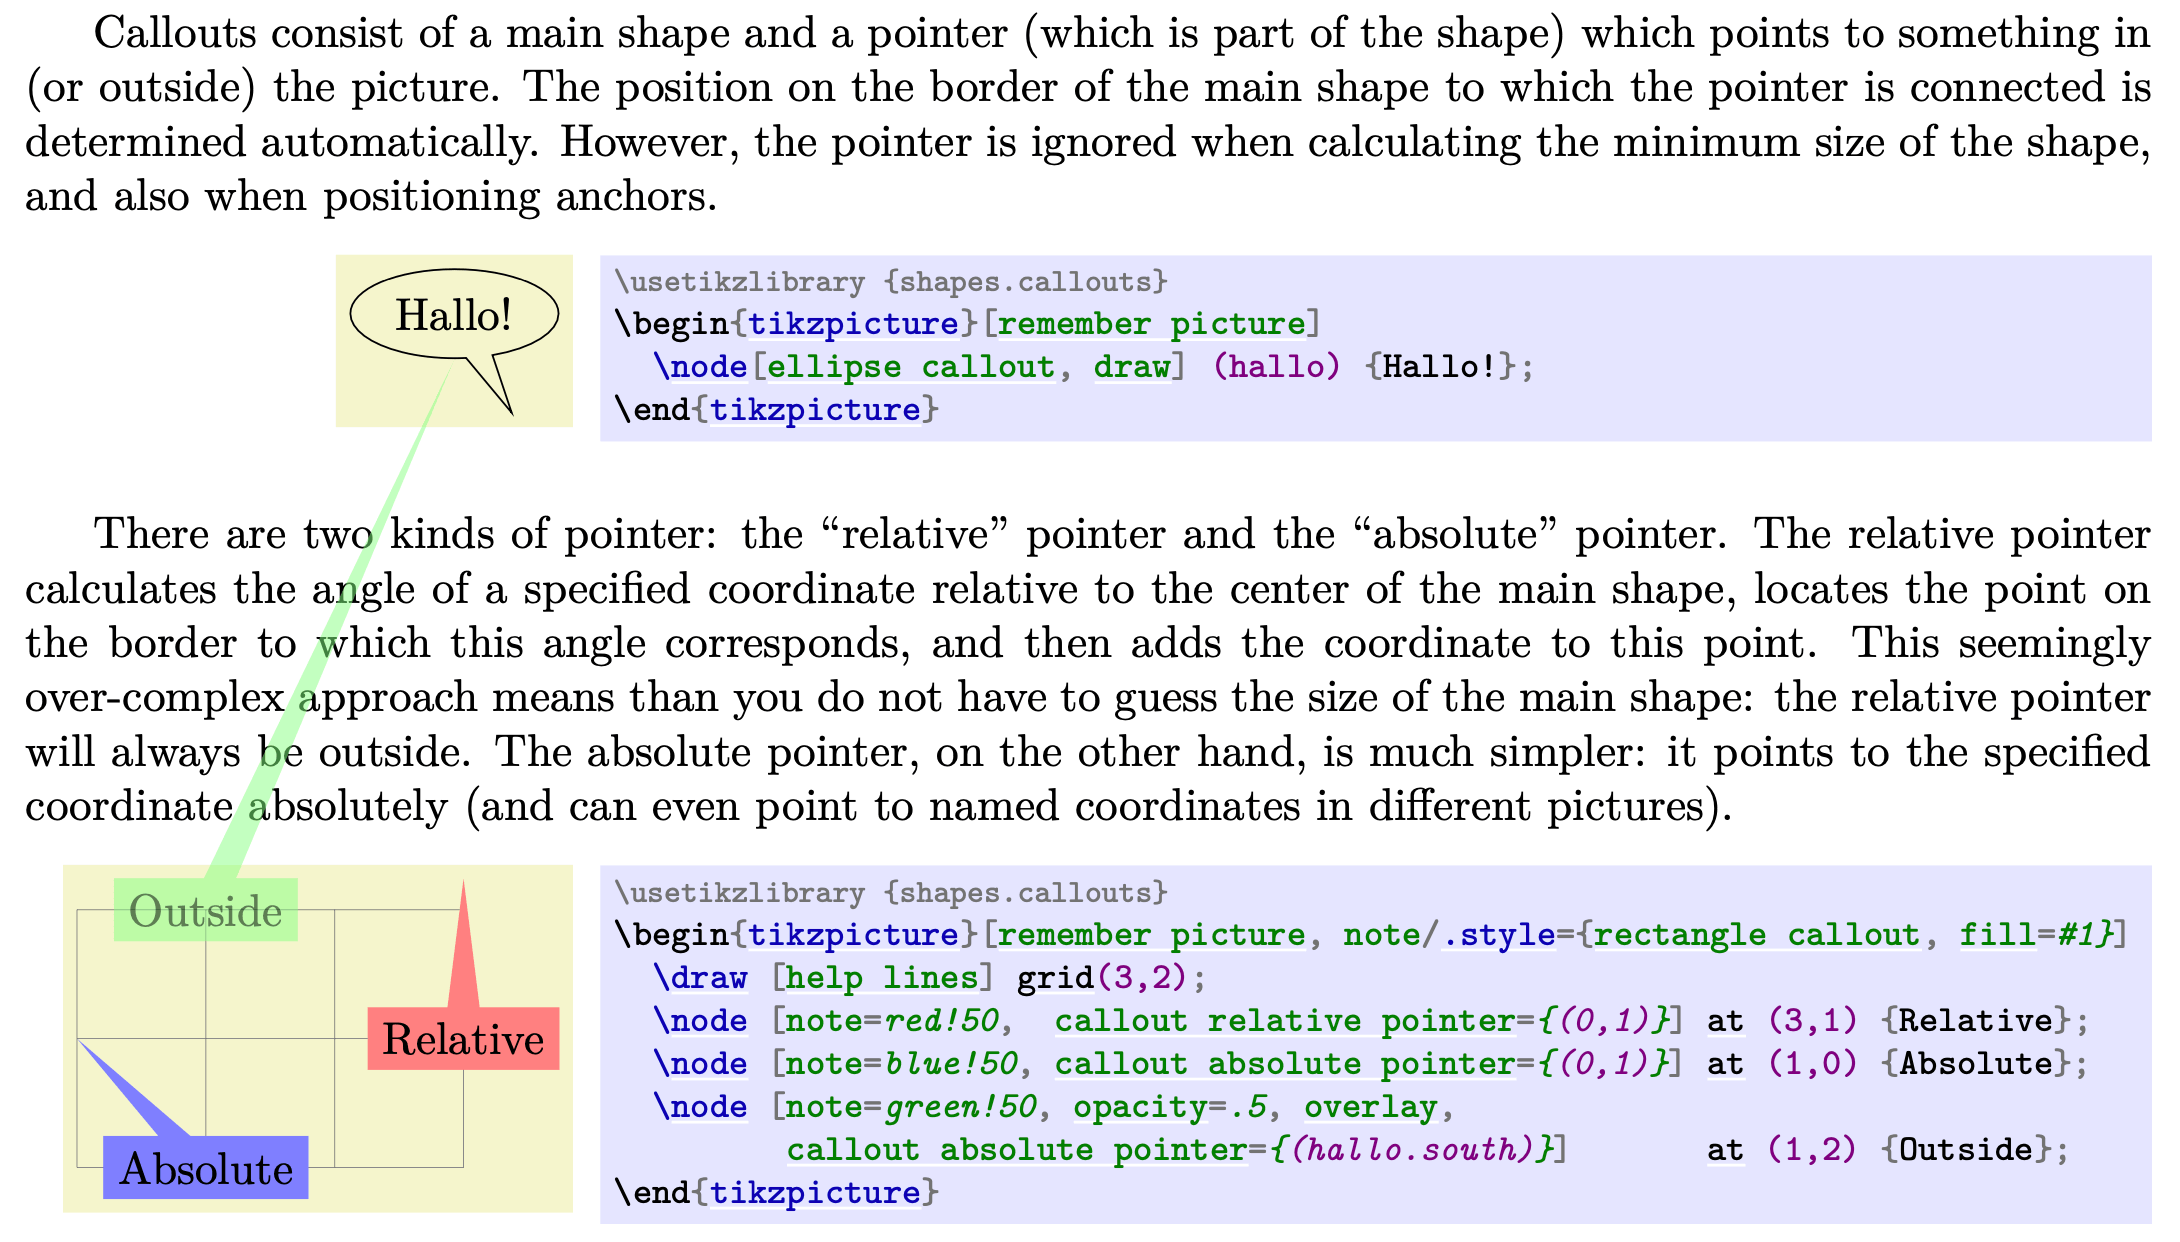
\includegraphics{standalone/pgfmanual-sec-71-7}
}

Callouts consist of a main shape and a pointer (which is part of the shape)
which points to something in (or outside) the picture. The position on the
border of the main shape to which the pointer is connected is determined
automatically. However, the pointer is ignored when calculating the minimum
size of the shape, and also when positioning anchors.
%
\begin{codeexample}[preamble={\usetikzlibrary{shapes.callouts}}]
\begin{tikzpicture}[remember picture]
  \node[ellipse callout, draw] (hallo) {Hallo!};
\end{tikzpicture}
\end{codeexample}

There are two kinds of pointer: the ``relative'' pointer and the ``absolute''
pointer. The relative pointer calculates the angle of a specified coordinate
relative to the center of the main shape, locates the point on the border to
which this angle corresponds, and then adds the coordinate to this point. This
seemingly over-complex approach means than you do not have to guess the size of
the main shape: the relative pointer will always be outside. The absolute
pointer, on the other hand, is much simpler: it points to the specified
coordinate absolutely (and can even point to named coordinates in different
pictures).
%
\begin{codeexample}[preamble={\usetikzlibrary{shapes.callouts}}]
\begin{tikzpicture}[remember picture, note/.style={rectangle callout, fill=#1}]
  \draw [help lines] grid(3,2);
  \node [note=red!50,  callout relative pointer={(0,1)}] at (3,1) {Relative};
  \node [note=blue!50, callout absolute pointer={(0,1)}] at (1,0) {Absolute};
  \node [note=green!50, opacity=.5, overlay,
         callout absolute pointer={(hallo.south)}]       at (1,2) {Outside};
\end{tikzpicture}
\end{codeexample}

The following keys are common to all callouts. Please remember that the
|callout| |relative| |pointer|, and |callout| |absolute| |pointer| keys take a
different format for their value depending on whether they are being used in
\pgfname{} or \tikzname{}.

\begin{key}{/pgf/callout relative pointer=\meta{coordinate} (initially {\ttfamily\char`\\pgfpointpolar\char`\{315\char`\}\char`\{.5cm\char`\}})}
    Sets the vector of the callout pointer `relative' to the callout shape.
\end{key}

\begin{key}{/pgf/callout absolute pointer=\meta{coordinate}}
    Sets the vector of the callout pointer absolutely within the picture.
\end{key}

\begin{key}{/tikz/callout relative pointer=\meta{coordinate} (initially {(315:.5cm)})}
    The \tikzname{} version of the |callout relative pointer| key. Here,
    \meta{coordinate} can be specified using the \tikzname{} format for
    coordinates.
\end{key}

\begin{key}{/tikz/callout absolute pointer=\meta{coordinate}}
    The \tikzname{} version of the |callout absolute pointer| key. Here,
    \meta{coordinate} can be specified using the \tikzname{} format for
    coordinates.
\end{key}

It is also possible to shorten the pointer by some distance, using the
following key:

\begin{key}{/pgf/callout pointer shorten=\meta{distance} (initially 0cm)}
    Moves the callout pointer towards the center of the callout's main shape by
    \meta{distance}.
    %
\begin{codeexample}[preamble={\usetikzlibrary{shapes.callouts}}]
\begin{tikzpicture}
    \tikzset{callout/.style={ellipse callout, callout pointer arc=30,
      callout absolute pointer={#1}}}
  \draw (0,0) grid (3,2);
  \node[callout={(3,1.5)}, fill=red!50] at (0,1.5) {A};
  \node[callout={(3,.5)},  fill=green!50, callout pointer shorten=1cm]
    at (0,.5)  {B};
\end{tikzpicture}
\end{codeexample}
    %
\end{key}

\begin{shape}{rectangle callout}
    This shape is a callout whose main shape is a rectangle, which tightly fits
    the node contents (including any |inner sep|). It supports the keys
    described above and also the following key:

    \begin{key}{/pgf/callout pointer width=\meta{length} (initially .25cm)}
        Sets the width of the pointer at the border of the rectangle.
    \end{key}

    The anchors for this shape are shown below (anchor |60| is an example of a
    border anchor). The pointer direction is ignored when placing anchors.
    Additionally, when using an absolute pointer, the |pointer| anchor should
    not to be used to used to position the shape as it is calculated whilst the
    shape is being drawn.
    %
\begin{codeexample}[preamble={\usetikzlibrary{shapes.callouts}}]
\Huge
\begin{tikzpicture}
  \node[name=s,shape=rectangle callout, callout relative pointer={(1.25cm,-1cm)},
     callout pointer width=2cm, shape example, inner xsep=2cm, inner ysep=1cm]
      {Rectangle Callout\vrule width 1pt height 2cm};
  \foreach \anchor/\placement in
    {center/above, text/below,      60/above,
     mid/right,    mid west/left,  mid east/right,
     base/below,   base west/below, base east/below,
     north/above,  south/below, east/above, west/above,
     north west/above, north east/above,
     south west/below, south east/below,
     pointer/below}
     \draw[shift=(s.\anchor)] plot[mark=x] coordinates{(0,0)}
       node[\placement] {\scriptsize\texttt{(s.\anchor)}};
\end{tikzpicture}
\end{codeexample}
    %
\end{shape}

\begin{shape}{ellipse callout}
    This shape is a callout whose main shape is an ellipse, which tightly fits
    the node contents (including any |inner sep|). It uses the
    |absolute callout pointer|, |relative callout pointer| and
    |callout pointer shorten| keys, and also the following key:

    \begin{key}{/pgf/callout pointer arc=\meta{angle} (initially 15)}
        Sets the width of the pointer at the border of the ellipse according to
        an arc of length \meta{angle}.
    \end{key}

    The anchors for this shape are shown below (anchor |60| is an example of a
    border anchor). The pointer direction is ignored when placing anchors and
    the |pointer| anchor can only be used to position the shape when the
    relative anchor is specified.
    %
\begin{codeexample}[preamble={\usetikzlibrary{shapes.callouts}}]
\Huge
\begin{tikzpicture}
  \node[name=s,shape=ellipse callout, callout relative pointer={(1.25cm,-1cm)},
    callout pointer width=2cm, shape example, inner xsep=1cm, inner ysep=.5cm]
      {Ellipse Callout\vrule width 1pt height 2cm};
  \foreach \anchor/\placement in
    {center/above, text/below,      60/above,
     mid/above,    mid west/right,  mid east/left,
     base/below,   base west/below, base east/below,
     north/above,  south/below, east/above, west/above,
     north west/above left,    north east/above right,
     south west/below left,    south east/below right,
     pointer/below}
     \draw[shift=(s.\anchor)] plot[mark=x] coordinates{(0,0)}
       node[\placement] {\scriptsize\texttt{(s.\anchor)}};
\end{tikzpicture}
\end{codeexample}
    %
\end{shape}

\begin{shape}{cloud callout}
    This shape is a callout whose main shape is a cloud which fits the node
    contents. The pointer is segmented, consisting of a series of shrinking
    ellipses. This callout requires the |shapes.callouts| library (for the cloud
    shape). If this library is not loaded an error will result.
    %
\begin{codeexample}[preamble={\usetikzlibrary{shapes.callouts}}]
\begin{tikzpicture}
  \node[cloud callout, cloud puffs=15, aspect=2.5, cloud puff arc=120,
    shading=ball,text=white] {\bf Imagine...};
\end{tikzpicture}
\end{codeexample}

    The |cloud callout| supports the |absolute callout pointer|,
    |relative callout pointer| and |callout pointer shorten| keys, as described
    above. The main shape can be modified using the same keys as the |cloud|
    shape. The following keys are also supported:

    \begin{key}{/pgf/callout pointer start size=\meta{value} (initially .2 of callout)}
        Sets the size of the first segment in the pointer (i.e., the segment
        nearest the main cloud shape). There are three possible forms for
        \meta{value}:
        %
        \begin{itemize}
            \item A single dimension (e.g., |5pt|), in which case the first
                ellipse will have equal diameters of 5pt.
            \item Two dimensions (e.g., |10pt and 2.5pt|), which sets the $x$
                and $y$ diameters of the first ellipse.
            \item A decimal fraction (e.g., |.2 of callout|), in which case the
                $x$ and $y$ diameters of the first ellipse will be set as
                fractions of the width and height of the main shape. The
                keyword |of callout| cannot be omitted.
        \end{itemize}
    \end{key}

    \begin{key}{/pgf/callout pointer end size=\meta{value} (initially .1 of callout)}
        Sets the size of the last ellipse in the pointer.
    \end{key}

    \begin{key}{/pgf/callout pointer segments=\meta{number} (initially 2)}
        Sets the number of segments in the pointer. Note that \pgfname{} will
        happily overlap segments if too many are specified.
    \end{key}

    The anchors for this shape are shown below (anchor |70| is an example of a
    border anchor). The pointer direction is ignored when placing anchors and
    the pointer anchor can only be used to position the shape when the relative
    anchor is specified. Note that the center of the last segment is drawn at
    the |pointer| anchor.
    %
\begin{codeexample}[preamble={\usetikzlibrary{shapes.callouts}}]
\Huge
\begin{tikzpicture}
  \node[name=s, shape=cloud callout, style=shape example, cloud puffs=11, aspect=1.5,
    cloud puff arc=120,inner xsep=.5cm, callout pointer start size=.25 of callout,
    callout pointer end size=.15 of callout, callout relative pointer={(315:4cm)},
    callout pointer segments=2] {Cloud Callout\vrule width 1pt height 2cm};
  \foreach \anchor/\placement in
    {puff 1/above, puff 2/above, puff 3/above, puff 4/below,
     puff 5/left, puff 6/below, puff 7/below, puff 8/right,
     puff 9/below, puff 10/above, puff 11/above, 70/right,
     center/above, base/below, mid/right, text/left,
     north/below, south/below, east/above, west/above,
     north west/left, north east/right,
     south west/below, south east/below,pointer/above}
  \draw[shift=(s.\anchor)] plot[mark=x] coordinates{(0,0)}
    node[\placement] {\scriptsize\texttt{(s.\anchor)}};
\end{tikzpicture}
\end{codeexample}
    %
\end{shape}


\subsection{Miscellaneous Shapes}

\begin{pgflibrary}{shapes.misc}
    This library defines general-purpose shapes that do not fit into the
    previous categories.
\end{pgflibrary}

\begin{shape}{cross out}
    This shape ``crosses out'' the node. Its foreground path are simply two
    diagonal lines between the corners of the node's bounding box. Here is an
    example:
    %
\begin{codeexample}[preamble={\usetikzlibrary{shapes.misc}}]
\begin{tikzpicture}
  \draw [help lines] (0,0) grid (3,2);
  \node [cross out,draw=red] at (1.5,1) {cross out};
\end{tikzpicture}
\end{codeexample}

    A useful application is inside text as in the following example:
    %
\begin{codeexample}[preamble={\usetikzlibrary{shapes.misc}}]
Cross \tikz[baseline] \node [cross out,draw,anchor=text] {me}; out!
\end{codeexample}

    This shape inherits all anchors from the |rectangle| shape, see also the
    following figure:
    %
\begin{codeexample}[preamble={\usetikzlibrary{shapes.misc}}]
\Huge
\begin{tikzpicture}
  \node[name=s,shape=cross out,shape example] {cross out\vrule width 1pt height 2cm};
  \foreach \anchor/\placement in
    {north west/above left, north/above, north east/above right,
     west/left, center/above, east/right,
     mid west/right, mid/above, mid east/left,
     base west/left, base/below, base east/right,
     south west/below left, south/below, south east/below right,
     text/left, 10/right, 130/above}
     \draw[shift=(s.\anchor)] plot[mark=x] coordinates{(0,0)}
       node[\placement] {\scriptsize\texttt{(s.\anchor)}};
\end{tikzpicture}
\end{codeexample}
    %
\end{shape}

\begin{shape}{strike out}
    This shape is identical to the |cross out| shape, only its foreground path
    consists of a single line from the lower left to the upper right.
    %
\begin{codeexample}[preamble={\usetikzlibrary{shapes.misc}}]
Strike \tikz[baseline] \node [strike out,draw,anchor=text] {me}; out!
\end{codeexample}

    See the |cross out| shape for the anchors.
\end{shape}

\begin{shape}{rounded rectangle}
    This shape is a rectangle which can have optionally rounded sides.
    %
\begin{codeexample}[preamble={\usetikzlibrary{shapes.misc}}]
\begin{tikzpicture}
  \node[rounded rectangle, draw, fill=red!20]{Hallo};
\end{tikzpicture}
\end{codeexample}

    There are keys to specify how the sides are rounded (to use these keys in
    \tikzname, simply remove the \declare{|/pgf/|} path).

    \begin{key}{/pgf/rounded rectangle arc length=\meta{angle} (initially 180)}
        Sets the length of the arcs for the rounded ends. Recommended values
        for \meta{angle} are between |90| and |180|.
        %
\begin{codeexample}[preamble={\usetikzlibrary{shapes.misc}}]
\begin{tikzpicture}
  \matrix[row sep=5pt, every node/.style={draw, rounded rectangle}]{
    \node[rounded rectangle arc length=180] {180}; \\
    \node[rounded rectangle arc length=120] {120}; \\
    \node[rounded rectangle arc length=90]  {90};  \\};
\end{tikzpicture}
\end{codeexample}
    \end{key}

    \begin{key}{/pgf/rounded rectangle west arc=\meta{arc type} (initially convex)}
        Sets the style of the rounding for the left side. The permitted values
        for \meta{arc type} are |concave|, |convex|, or |none|.
        %
\begin{codeexample}[preamble={\usetikzlibrary{shapes.misc}}]
\begin{tikzpicture}
  \matrix[row sep=5pt, every node/.style={draw, rounded rectangle}]{
    \node[rounded rectangle west arc=concave] {Concave}; \\
    \node[rounded rectangle west arc=convex]  {Convex};  \\
    \node[rounded rectangle left arc=none]    {None};    \\};
\end{tikzpicture}
\end{codeexample}
    \end{key}

    \begin{stylekey}{/pgf/rounded rectangle left arc=\meta{arc type}}
        Alternative key for specifying the west arc.
    \end{stylekey}

    \begin{key}{/pgf/rounded rectangle east arc=\meta{arc type} (initially convex)}
        Sets the style of the rounding for the east side.
    \end{key}

    \begin{stylekey}{/pgf/rounded rectangle right arc=\meta{arc type}}
        Alternative key for specifying the east arc.
    \end{stylekey}

    The anchors for this shape are shown below (anchor |10| is an example of a
    border angle). Note that if only one side is rounded, the |center| anchor
    will not be the precise center of the shape.
    %
\begin{codeexample}[preamble={\usetikzlibrary{shapes.misc}}]
\Huge
\begin{tikzpicture}
  \node[name=s,shape=rounded rectangle, shape example, inner xsep=1.5cm, inner ysep=1cm]
      {Rounded Rectangle\vrule width 1pt height 2cm};
  \foreach \anchor/\placement in
    {center/above, text/below,      10/above,
     mid/above,    mid west/right,  mid east/left,
     base/below,   base west/below, base east/below,
     north/above,  south/below, east/above, west/above,
     north west/above left,    north east/above right,
     south west/below left,    south east/below right}
     \draw[shift=(s.\anchor)] plot[mark=x] coordinates{(0,0)}
       node[\placement] {\scriptsize\texttt{(s.\anchor)}};
\end{tikzpicture}
\end{codeexample}
    %
\end{shape}

\begin{shape}{chamfered rectangle}
    This shape is a rectangle with optionally chamfered corners.
    %
\begin{codeexample}[preamble={\usetikzlibrary{shapes.misc}}]
\begin{tikzpicture}
  \node[chamfered rectangle, white, fill=red, double=red, draw, very thick]
    {\bf STOP!};
\end{tikzpicture}
\end{codeexample}

    There are \pgfname{} keys to specify how this shape is drawn (to use these
    keys in \tikzname{} simply remove the \declare{|/pgf/|} path).

    \begin{key}{/pgf/chamfered rectangle angle=\meta{angle} (initially 45)}
        Sets the angle \emph{from the vertical} for the chamfer.
        %
\begin{codeexample}[preamble={\usetikzlibrary{shapes.misc}}]
\begin{tikzpicture}
  \tikzset{every node/.style={chamfered rectangle, draw}}
  \node[chamfered rectangle angle=30] {abc};
  \node[chamfered rectangle angle=60] at (1.5,0) {123};
\end{tikzpicture}
\end{codeexample}
    \end{key}

    \begin{key}{/pgf/chamfered rectangle xsep=\meta{length} (initially .666ex)}
        Sets the distance that the chamfer extends horizontally beyond the node
        contents (which includes the |inner sep|). If \meta{length} is large,
        such that the top and bottom chamfered edges would cross, then
        \meta{length} is ignored and the chamfered edges are drawn so that they
        meet in the middle.
        %
\begin{codeexample}[preamble={\usetikzlibrary{shapes.misc}}]
\begin{tikzpicture}
  \tikzset{every node/.style={chamfered rectangle, draw}}
  \node[chamfered rectangle xsep=2pt] {def};
  \node[chamfered rectangle xsep=2cm] at (1.5,0) {456};
\end{tikzpicture}
\end{codeexample}
    \end{key}

    \begin{key}{/pgf/chamfered rectangle ysep=\meta{length} (initially .666ex)}
        Sets the distance that the chamfer extends vertically beyond the node
        contents. If \meta{length} is large, such that the left and right
        chamfered edges would cross, then \meta{length} is ignored and the
        chamfered edges are drawn so that they meet in the middle.
    \end{key}

    \begin{key}{/pgf/chamfered rectangle sep=\meta{length} (initially .666ex)}
        Sets both the |xsep| and |ysep| simultaneously.
    \end{key}

    \begin{key}{/pgf/chamfered rectangle corners=\meta{list} (initially chamfer all)}
        Specifies which corners are chamfered. The corners are identified by
        their ``compass point'' directions (i.e.\ |north east|, |north west|,
        |south west|, and |south east|), and must be separated by commas (so if
        there is more than one corner in the list, it must be surrounded by
        braces). Any corners not mentioned in \meta{list} are automatically not
        chamfered. Two additional values |chamfer all| and |chamfer none|, are
        also permitted.
        %
\begin{codeexample}[preamble={\usetikzlibrary{shapes.misc}}]
\begin{tikzpicture}
  \tikzset{every node/.style={chamfered rectangle, draw}}
  \node[chamfered rectangle corners=north west] {ghi};
  \node[chamfered rectangle corners={north east, south east}] at (1.5,0) {789};
\end{tikzpicture}
\end{codeexample}
    \end{key}

    The anchors for this shape are shown below (anchor |60| is an example of a
    border angle.
    %
\begin{codeexample}[preamble={\usetikzlibrary{shapes.misc}}]
\Huge
\begin{tikzpicture}
  \node[name=s,shape=chamfered rectangle, chamfered rectangle sep=1cm,
        shape example, inner ysep=1cm, inner xsep=.75cm]
    {Chamfered Rectangle\vrule width1pt height2cm};
  \foreach \anchor/\placement in
    {text/right, center/above,    70/above,
     base/below, base east/left, base west/right,
     mid/right,  mid east/above,   mid west/above,
     north/above, south/below, east/above, west/above,
     before north east/above, north east/above, after north east/above,
     before north west/above, north west/above, after north west/above,
     before south west/below, south west/below, after south west/below,
     before south east/below, south east/below, after south east/below}
     \draw[shift=(s.\anchor)] plot[mark=x] coordinates{(0,0)}
       node[\placement] {\scriptsize\texttt{(s.\anchor)}};
\end{tikzpicture}
\end{codeexample}
    %
\end{shape}


%%% Local Variables:
%%% mode: latex
%%% TeX-master: "pgfmanual-pdftex-version"
%%% End:
